\documentclass{article}
\usepackage[preprint]{neurips_2026}
\usepackage[utf8]{inputenc}
\usepackage[T1]{fontenc}
\usepackage{hyperref,url,booktabs,amsfonts,amsmath,amssymb,amsthm,nicefrac,microtype,xcolor,graphicx}
\usepackage[section]{placeins}  % floats never cross a section boundary (nor into the checklist)
\newtheorem{proposition}{Proposition}\newtheorem{remark}{Remark}
\newcommand{\todo}[1]{\textcolor{red}{[TODO: #1]}}
\newcommand{\HRR}{\mathrm{HRR}}\newcommand{\BRR}{\mathrm{BRR}}\newcommand{\SRR}{\mathrm{SRR}}
\newcommand{\ci}[2]{{\small[$#1$, $#2$]}}
% AUTO-GENERATED by src/paper_numbers.py — do not edit by hand.

\newcommand{\RefKappaMean}{0.93}  % runs/pgp_val/judge_validation.csv (Gemini-3.5-Flash broad)
\newcommand{\RefKappaMin}{0.92}  % runs/pgp_val/judge_validation.csv (Gemini-3.5-Flash broad)
\newcommand{\RefAccMean}{97\%}  % runs/pgp_val/judge_validation.csv (Gemini-3.5-Flash broad)
\newcommand{\HarmKappaMean}{0.43}  % runs/pgp_val/judge_validation.csv (Gemini-3.5-Flash broad)
\newcommand{\HarmMissSplit}{90\%}  % runs/pgp_val/gemini_broad_judged.jsonl
\newcommand{\HarmMissUnanimous}{41\%}  % runs/pgp_val/gemini_broad_judged.jsonl
\newcommand{\RefAccUnanimous}{97.8\%}  % runs/pgp_val/gemini_broad_judged.jsonl
\newcommand{\NValidation}{1,400}  % runs/pgp_val/gemini_broad_judged.jsonl
\newcommand{\QRefKappaMean}{0.89}  % runs/pgp_val/judge_validation.csv (Qwen3Guard-4B)
\newcommand{\QHarmKappaMean}{0.74}  % runs/pgp_val/judge_validation.csv (Qwen3Guard-4B)
\newcommand{\QHarmKappaMin}{0.70}  % runs/pgp_val/judge_validation.csv (Qwen3Guard-4B)
\newcommand{\QHarmKappaMax}{0.77}  % runs/pgp_val/judge_validation.csv (Qwen3Guard-4B)
\newcommand{\QHarmMiss}{29\%}  % runs/pgp_val/judge_validation.csv (Qwen3Guard-4B)
\newcommand{\GemHarmMiss}{63\%}  % runs/pgp_val/judge_validation.csv (Gemini broad)
\newcommand{\QUnparseable}{5}  % runs/pgp_val/judged.jsonl x human labels (gemini_broad_judged.jsonl)
\newcommand{\QHarmMissSplit}{54\%}  % runs/pgp_val/judged.jsonl x human labels (gemini_broad_judged.jsonl)
\newcommand{\QHarmMissUnanimous}{9\%}  % runs/pgp_val/judged.jsonl x human labels (gemini_broad_judged.jsonl)
\newcommand{\RefAccMeanTxt}{97\%}  % runs/pgp_val/judge_validation.csv (Gemini broad)
\newcommand{\GemHRRMin}{46\%}  % runs/GEM-lite/judged.jsonl via analyze.load(judge=gem)
\newcommand{\GemHRRMax}{58\%}  % runs/GEM-lite/judged.jsonl via analyze.load(judge=gem)
\newcommand{\GemHarmMax}{1.9\%}  % runs/GEM-lite/judged.jsonl via analyze.load(judge=gem)
\newcommand{\GemHarmMean}{0.7\%}  % runs/GEM-lite/judged.jsonl via analyze.load(judge=gem)
\newcommand{\GemGSrr}{99.3\%}  % runs/GEM-lite/judged.jsonl via analyze.load(judge=gem)
\newcommand{\BZeroQRefHrl}{69\%}  % figures.outcome_table('B0', 'q3g4b') on runs/B0/judged.jsonl
\newcommand{\BZeroQRefLrl}{52\%}  % figures.outcome_table('B0', 'q3g4b') on runs/B0/judged.jsonl
\newcommand{\BZeroQHarmHrl}{4.3\%}  % figures.outcome_table('B0', 'q3g4b') on runs/B0/judged.jsonl
\newcommand{\BZeroQHarmLrl}{4.3\%}  % figures.outcome_table('B0', 'q3g4b') on runs/B0/judged.jsonl
\newcommand{\BZeroQHarmMean}{4.6\%}  % figures.outcome_table('B0', 'q3g4b') on runs/B0/judged.jsonl
\newcommand{\BZeroQHarmMax}{8\%}  % figures.outcome_table('B0', 'q3g4b') on runs/B0/judged.jsonl
\newcommand{\BZeroQBrrTh}{23\%}  % figures.outcome_table('B0', 'q3g4b') on runs/B0/judged.jsonl
\newcommand{\BZeroQBrrJv}{17\%}  % figures.outcome_table('B0', 'q3g4b') on runs/B0/judged.jsonl
\newcommand{\BZeroQBrrMean}{12.8\%}  % figures.outcome_table('B0', 'q3g4b') on runs/B0/judged.jsonl
\newcommand{\BZeroGRefHrl}{67\%}  % figures.outcome_table('B0', 'gem') on runs/B0/judged.jsonl
\newcommand{\BZeroGRefLrl}{57\%}  % figures.outcome_table('B0', 'gem') on runs/B0/judged.jsonl
\newcommand{\BZeroGHarmHrl}{1.8\%}  % figures.outcome_table('B0', 'gem') on runs/B0/judged.jsonl
\newcommand{\BZeroGHarmLrl}{4.5\%}  % figures.outcome_table('B0', 'gem') on runs/B0/judged.jsonl
\newcommand{\BZeroGHarmMean}{3.6\%}  % figures.outcome_table('B0', 'gem') on runs/B0/judged.jsonl
\newcommand{\BZeroGHarmMax}{6\%}  % figures.outcome_table('B0', 'gem') on runs/B0/judged.jsonl
\newcommand{\BZeroGBrrTh}{23\%}  % figures.outcome_table('B0', 'gem') on runs/B0/judged.jsonl
\newcommand{\BZeroGBrrJv}{18\%}  % figures.outcome_table('B0', 'gem') on runs/B0/judged.jsonl
\newcommand{\BZeroGBrrMean}{10.6\%}  % figures.outcome_table('B0', 'gem') on runs/B0/judged.jsonl
\newcommand{\BZeroGemHarmRatio}{5}  % B0 mean harm (gem judge) / GEM-lite mean harm
\newcommand{\HOneGap}{0.86}  % runs/B0/h1.json (src/h1.py)
\newcommand{\HOneGapLo}{0.80}  % runs/B0/h1.json (src/h1.py)
\newcommand{\HOneGapHi}{0.92}  % runs/B0/h1.json (src/h1.py)
\newcommand{\HOneKappaEnMin}{0.85}  % runs/B0/h1.json (src/h1.py)
\newcommand{\HOneKappaEnMax}{0.92}  % runs/B0/h1.json (src/h1.py)
\newcommand{\HOneKappaOtherMax}{0.00}  % runs/B0/h1.json (src/h1.py)
\newcommand{\HOneRecallOtherMax}{0\%}  % runs/B0/h1.json (src/h1.py)
\newcommand{\FailN}{134}  % runs/B0/gate_on_failures.json (src/failure_gate.py)
\newcommand{\FailEors}{95\%}  % runs/B0/gate_on_failures.json (src/failure_gate.py)
\newcommand{\FailEorsLo}{90\%}  % runs/B0/gate_on_failures.json (src/failure_gate.py)
\newcommand{\FailEorsHi}{97\%}  % runs/B0/gate_on_failures.json (src/failure_gate.py)
\newcommand{\FailSingle}{95\%}  % runs/B0/gate_on_failures.json (src/failure_gate.py)
\newcommand{\FailRefusedEors}{95\%}  % runs/B0/gate_on_failures.json (src/failure_gate.py)
\newcommand{\FailThK}{8}  % runs/B0/gate_on_failures.json (src/failure_gate.py)
\newcommand{\FailThN}{10}  % runs/B0/gate_on_failures.json (src/failure_gate.py)
\newcommand{\RoiGemN}{3,950}  % runs/GEM-lite/responses.jsonl usage_metadata x list price
\newcommand{\RoiGemCost}{\$1.71}  % runs/GEM-lite/responses.jsonl usage_metadata x list price
\newcommand{\RoiGemPerK}{\$0.43}  % runs/GEM-lite/responses.jsonl usage_metadata x list price
\newcommand{\RoiGemMeanOut}{171}  % runs/GEM-lite/responses.jsonl usage_metadata x list price
\newcommand{\RoiGemPerKCap}{\$0.25}  % runs/GEM-lite/responses.jsonl usage_metadata x list price (96-token cap)
\newcommand{\RoiTinyPerMin}{27}  % runs/roi_timing.json (B0, E0 generation wall time)
\newcommand{\RoiTinyHoursPerM}{615}  % runs/roi_timing.json (B0, E0 generation wall time)
\newcommand{\GemBrrMean}{1.9\%}  % analyze.summary(GEM-lite, judge=gem), ten languages
\newcommand{\DriftQSrr}{-1.1}  % analyze.compare(B0, E0, judge=q3g4b) paired bootstrap / McNemar-Holm
\newcommand{\DriftQSrrLo}{-1.9}  % analyze.compare(B0, E0, judge=q3g4b) paired bootstrap / McNemar-Holm
\newcommand{\DriftQSrrHi}{-0.3}  % analyze.compare(B0, E0, judge=q3g4b) paired bootstrap / McNemar-Holm
\newcommand{\DriftQWorstSrr}{-3.8}  % analyze.compare(B0, E0, judge=q3g4b) paired bootstrap / McNemar-Holm
\newcommand{\DriftQWorstSrrLo}{-7.2}  % analyze.compare(B0, E0, judge=q3g4b) paired bootstrap / McNemar-Holm
\newcommand{\DriftQWorstSrrHi}{+1.0}  % analyze.compare(B0, E0, judge=q3g4b) paired bootstrap / McNemar-Holm
\newcommand{\DriftQHrr}{-3.5}  % analyze.compare(B0, E0, judge=q3g4b) paired bootstrap / McNemar-Holm
\newcommand{\DriftQHrrLo}{-4.9}  % analyze.compare(B0, E0, judge=q3g4b) paired bootstrap / McNemar-Holm
\newcommand{\DriftQHrrHi}{-2.1}  % analyze.compare(B0, E0, judge=q3g4b) paired bootstrap / McNemar-Holm
\newcommand{\DriftQMaxBrr}{-2.8}  % analyze.compare(B0, E0, judge=q3g4b) paired bootstrap / McNemar-Holm
\newcommand{\DriftQMaxBrrLo}{-8.5}  % analyze.compare(B0, E0, judge=q3g4b) paired bootstrap / McNemar-Holm
\newcommand{\DriftQMaxBrrHi}{+2.8}  % analyze.compare(B0, E0, judge=q3g4b) paired bootstrap / McNemar-Holm
\newcommand{\DriftQNSig}{0}  % analyze.compare(B0, E0, judge=q3g4b) paired bootstrap / McNemar-Holm
\newcommand{\DriftQHarmBn}{+3.8}  % analyze.compare(B0, E0, judge=q3g4b) paired bootstrap / McNemar-Holm
\newcommand{\DriftGSrr}{-1.0}  % analyze.compare(B0, E0, judge=gem) paired bootstrap / McNemar-Holm
\newcommand{\DriftGSrrLo}{-1.9}  % analyze.compare(B0, E0, judge=gem) paired bootstrap / McNemar-Holm
\newcommand{\DriftGSrrHi}{-0.2}  % analyze.compare(B0, E0, judge=gem) paired bootstrap / McNemar-Holm
\newcommand{\DriftGWorstSrr}{-2.9}  % analyze.compare(B0, E0, judge=gem) paired bootstrap / McNemar-Holm
\newcommand{\DriftGWorstSrrLo}{-5.8}  % analyze.compare(B0, E0, judge=gem) paired bootstrap / McNemar-Holm
\newcommand{\DriftGWorstSrrHi}{+1.9}  % analyze.compare(B0, E0, judge=gem) paired bootstrap / McNemar-Holm
\newcommand{\DriftGHrr}{-3.3}  % analyze.compare(B0, E0, judge=gem) paired bootstrap / McNemar-Holm
\newcommand{\DriftGHrrLo}{-4.7}  % analyze.compare(B0, E0, judge=gem) paired bootstrap / McNemar-Holm
\newcommand{\DriftGHrrHi}{-1.8}  % analyze.compare(B0, E0, judge=gem) paired bootstrap / McNemar-Holm
\newcommand{\DriftGMaxBrr}{-6.6}  % analyze.compare(B0, E0, judge=gem) paired bootstrap / McNemar-Holm
\newcommand{\DriftGMaxBrrLo}{-12.3}  % analyze.compare(B0, E0, judge=gem) paired bootstrap / McNemar-Holm
\newcommand{\DriftGMaxBrrHi}{-0.9}  % analyze.compare(B0, E0, judge=gem) paired bootstrap / McNemar-Holm
\newcommand{\DriftGNSig}{0}  % analyze.compare(B0, E0, judge=gem) paired bootstrap / McNemar-Holm
\newcommand{\DriftGHarmBn}{+4.3}  % analyze.compare(B0, E0, judge=gem) paired bootstrap / McNemar-Holm
\newcommand{\ReportMinSafeGlobal}{87.0}  % Salamanca et al. 2026 (arXiv 2603.11510v1) Table 7, read 2026-10-27
\newcommand{\ReportMinSafeEarth}{77.5}  % Salamanca et al. 2026 (arXiv 2603.11510v1) Table 7, read 2026-10-27
\newcommand{\ReportMeanSafeGlobal}{91.1}  % Salamanca et al. 2026 (arXiv 2603.11510v1) Table 7, read 2026-10-27
\newcommand{\ReportMeanSafeEarth}{87.8}  % Salamanca et al. 2026 (arXiv 2603.11510v1) Table 7, read 2026-10-27
\newcommand{\ReportMinSafeDrop}{9.5}  % Salamanca et al. 2026 (arXiv 2603.11510v1) Table 7, read 2026-10-27
\newcommand{\PowerNHarm}{209}  % analyze.load(B0, E0, judge=q3g4b) discordance + Connor (1987) McNemar MDE, 80% power
\newcommand{\PowerPsiHarm}{3.8\%}  % analyze.load(B0, E0, judge=q3g4b) discordance + Connor (1987) McNemar MDE, 80% power
\newcommand{\PowerMdeHarm}{3.8 points}  % analyze.load(B0, E0, judge=q3g4b) discordance + Connor (1987) McNemar MDE, 80% power
\newcommand{\PowerMdeHarmHolm}{not attainable}  % analyze.load(B0, E0, judge=q3g4b) discordance + Connor (1987) McNemar MDE, 80% power
\newcommand{\PowerNBrr}{106}  % analyze.load(B0, E0, judge=q3g4b) discordance + Connor (1987) McNemar MDE, 80% power
\newcommand{\PowerPsiBrr}{6.6\%}  % analyze.load(B0, E0, judge=q3g4b) discordance + Connor (1987) McNemar MDE, 80% power
\newcommand{\PowerMdeBrr}{not attainable}  % analyze.load(B0, E0, judge=q3g4b) discordance + Connor (1987) McNemar MDE, 80% power
\newcommand{\PowerMdeBrrHolm}{not attainable}  % analyze.load(B0, E0, judge=q3g4b) discordance + Connor (1987) McNemar MDE, 80% power
\newcommand{\HThreeLayer}{14}  % runs/E0/h3.json (global_best layer, odd calibration half)
\newcommand{\HThreeDeficit}{Bengali, English, Swahili}  % runs/E0/h3.json (global_best layer, odd calibration half)
\newcommand{\HThreeAurocDropMax}{0.009}  % runs/E0/h3.json (global_best layer, odd calibration half)
\newcommand{\HThreeDBnChange}{+0.10}  % runs/E0/h3.json (global_best layer, odd calibration half)
\newcommand{\HThreeDSwChange}{+0.13}  % runs/E0/h3.json (global_best layer, odd calibration half)
\newcommand{\HThreeDEnChange}{-0.10}  % runs/E0/h3.json (global_best layer, odd calibration half)
\newcommand{\CkParityMaxKl}{3.5\times10^{-5}}  % runs/circuitkit/parity/parity_kaggle_v7_patched.json
\newcommand{\CkParityTopOne}{100\%}  % runs/circuitkit/parity/parity_kaggle_v7_patched.json
\newcommand{\CkParityN}{12}  % runs/circuitkit/parity/parity_kaggle_v7_patched.json
\newcommand{\BestLayer}{17}  % runs/mech_global/summary.json
\newcommand{\AurocMinNonJv}{0.96}  % runs/mech_global/summary.json
\newcommand{\AurocMax}{0.99}  % runs/mech_global/summary.json
\newcommand{\AurocJv}{0.91}  % runs/mech_global/summary.json
\newcommand{\CosMean}{0.79}  % runs/mech_global/summary.json
\newcommand{\CastPearson}{0.89}  % runs/mech_global/gate_proxy.json (h6)
\newcommand{\CastAurocSwProj}{0.97}  % runs/mech_global/gate_proxy.json (h6)
\newcommand{\CastAurocSwCast}{0.74}  % runs/mech_global/gate_proxy.json (h6)
\newcommand{\NegBenignZh}{6\%}  % runs/mech_global/gate_proxy.json (h6)
\newcommand{\NegBenignSw}{62\%}  % runs/mech_global/gate_proxy.json (h6)
\newcommand{\CastFprMin}{40\%}  % runs/mech_global/gate_proxy.json (h6)
\newcommand{\CastFprMax}{53\%}  % runs/mech_global/gate_proxy.json (h6)
\newcommand{\CondLayer}{14}  % runs/mech_global/gate_proxy.json (h6)
\newcommand{\MatchMeanFprSingle}{10.0\%}  % gate_proxy.matched_comparison(eps=0.10) on runs/mech_global
\newcommand{\MatchMeanFprEors}{11.5\%}  % gate_proxy.matched_comparison(eps=0.10) on runs/mech_global
\newcommand{\MatchMaxFprSingle}{30\%}  % gate_proxy.matched_comparison(eps=0.10) on runs/mech_global
\newcommand{\MatchMaxFprEors}{15\%}  % gate_proxy.matched_comparison(eps=0.10) on runs/mech_global
\newcommand{\MatchGapSingle}{29}  % gate_proxy.matched_comparison(eps=0.10) on runs/mech_global
\newcommand{\MatchGapEors}{9}  % gate_proxy.matched_comparison(eps=0.10) on runs/mech_global
\newcommand{\MatchThFprSingle}{30\%}  % gate_proxy.matched_comparison(eps=0.10) on runs/mech_global
\newcommand{\MatchThFprEors}{12\%}  % gate_proxy.matched_comparison(eps=0.10) on runs/mech_global
\newcommand{\MatchThTprSingle}{0.94}  % gate_proxy.matched_comparison(eps=0.10) on runs/mech_global
\newcommand{\MatchThTprEors}{0.78}  % gate_proxy.matched_comparison(eps=0.10) on runs/mech_global
\newcommand{\MatchHrlFprSingleMax}{4\%}  % gate_proxy.matched_comparison(eps=0.10) on runs/mech_global
\newcommand{\MatchHrlFprEorsMin}{11\%}  % gate_proxy.matched_comparison(eps=0.10) on runs/mech_global
\newcommand{\MatchHrlFprEorsMax}{15\%}  % gate_proxy.matched_comparison(eps=0.10) on runs/mech_global
\newcommand{\MatchMeanTprSingle}{0.92}  % gate_proxy.matched_comparison(eps=0.10) on runs/mech_global
\newcommand{\MatchMeanTprEors}{0.93}  % gate_proxy.matched_comparison(eps=0.10) on runs/mech_global
\newcommand{\EorsQMaxBrr}{-24.5}  % runs/arms_report.json (q3g4b)
\newcommand{\EorsQMaxBrrLo}{-34.9}  % runs/arms_report.json (q3g4b)
\newcommand{\EorsQMaxBrrHi}{-17.0}  % runs/arms_report.json (q3g4b)
\newcommand{\EorsQHrr}{-8.3}  % runs/arms_report.json (q3g4b)
\newcommand{\EorsQHrrLo}{-10.1}  % runs/arms_report.json (q3g4b)
\newcommand{\EorsQHrrHi}{-6.5}  % runs/arms_report.json (q3g4b)
\newcommand{\EorsQSrr}{-0.8}  % runs/arms_report.json (q3g4b)
\newcommand{\EorsQSrrLo}{-1.3}  % runs/arms_report.json (q3g4b)
\newcommand{\EorsQSrrHi}{-0.3}  % runs/arms_report.json (q3g4b)
\newcommand{\EorsTenQMaxBrr}{-19.8}  % runs/arms_report.json (q3g4b)
\newcommand{\EorsTenQMaxBrrLo}{-28.3}  % runs/arms_report.json (q3g4b)
\newcommand{\EorsTenQMaxBrrHi}{-12.3}  % runs/arms_report.json (q3g4b)
\newcommand{\CastQLrlHrr}{-3.0}  % runs/arms_report.json (q3g4b)
\newcommand{\CastQLrlHrrLo}{-4.6}  % runs/arms_report.json (q3g4b)
\newcommand{\CastQLrlHrrHi}{-1.8}  % runs/arms_report.json (q3g4b)
\newcommand{\CastQLrlUnsafe}{+0.2}  % runs/arms_report.json (q3g4b)
\newcommand{\CastQLrlUnsafeLo}{+0.0}  % runs/arms_report.json (q3g4b)
\newcommand{\CastQLrlUnsafeHi}{+0.5}  % runs/arms_report.json (q3g4b)
\newcommand{\PreQSrr}{+0.0}  % runs/arms_report.json (q3g4b)
\newcommand{\PreQSrrLo}{-0.6}  % runs/arms_report.json (q3g4b)
\newcommand{\PreQSrrHi}{+0.7}  % runs/arms_report.json (q3g4b)
\newcommand{\PreQHrr}{+1.5}  % runs/arms_report.json (q3g4b)
\newcommand{\PreQHrrLo}{+0.3}  % runs/arms_report.json (q3g4b)
\newcommand{\PreQHrrHi}{+2.8}  % runs/arms_report.json (q3g4b)
\newcommand{\RestaQSrr}{+0.4}  % runs/arms_report.json (q3g4b)
\newcommand{\RestaQSrrLo}{-1.0}  % runs/arms_report.json (q3g4b)
\newcommand{\RestaQSrrHi}{+1.9}  % runs/arms_report.json (q3g4b)
\newcommand{\RestaQMaxBrr}{+26.4}  % runs/arms_report.json (q3g4b)
\newcommand{\RestaQMaxBrrLo}{+17.0}  % runs/arms_report.json (q3g4b)
\newcommand{\RestaQMaxBrrHi}{+34.9}  % runs/arms_report.json (q3g4b)
\newcommand{\NegQSrr}{-4.9}  % runs/arms_report.json (q3g4b)
\newcommand{\NegQSrrLo}{-6.2}  % runs/arms_report.json (q3g4b)
\newcommand{\NegQSrrHi}{-3.6}  % runs/arms_report.json (q3g4b)
\newcommand{\ArmsQSrrGainMin}{+4.5}  % runs/arms_report.json (q3g4b)
\newcommand{\ArmsQSrrGainMax}{+5.6}  % runs/arms_report.json (q3g4b)
\newcommand{\ArmsQMaxBrrMin}{+22.6}  % runs/arms_report.json (q3g4b)
\newcommand{\ArmsQMaxBrrMax}{+31.1}  % runs/arms_report.json (q3g4b)
\newcommand{\EorsVsEQMaxBrr}{+6.6}  % runs/arms_report.json (q3g4b)
\newcommand{\CastPowerPsi}{1.9\%}  % runs/arms_report.json (q3g4b)
\newcommand{\CastPowerMde}{no per-language effect is detectable with 80\% power}  % runs/arms_report.json (q3g4b)
\newcommand{\CastNSig}{0}  % runs/arms_report.json (q3g4b)
\newcommand{\EorsGMaxBrr}{-22.6}  % runs/arms_report.json (gem)
\newcommand{\EorsGMaxBrrLo}{-33.0}  % runs/arms_report.json (gem)
\newcommand{\EorsGMaxBrrHi}{-16.0}  % runs/arms_report.json (gem)
\newcommand{\EorsGHrr}{-8.4}  % runs/arms_report.json (gem)
\newcommand{\EorsGHrrLo}{-10.3}  % runs/arms_report.json (gem)
\newcommand{\EorsGHrrHi}{-6.6}  % runs/arms_report.json (gem)
\newcommand{\EorsGSrr}{-0.5}  % runs/arms_report.json (gem)
\newcommand{\EorsGSrrLo}{-1.0}  % runs/arms_report.json (gem)
\newcommand{\EorsGSrrHi}{-0.2}  % runs/arms_report.json (gem)
\newcommand{\EorsTenGMaxBrr}{-18.9}  % runs/arms_report.json (gem)
\newcommand{\EorsTenGMaxBrrLo}{-27.2}  % runs/arms_report.json (gem)
\newcommand{\EorsTenGMaxBrrHi}{-13.2}  % runs/arms_report.json (gem)
\newcommand{\CastGLrlHrr}{-2.6}  % runs/arms_report.json (gem)
\newcommand{\CastGLrlHrrLo}{-4.1}  % runs/arms_report.json (gem)
\newcommand{\CastGLrlHrrHi}{-1.3}  % runs/arms_report.json (gem)
\newcommand{\CastGLrlUnsafe}{+0.3}  % runs/arms_report.json (gem)
\newcommand{\CastGLrlUnsafeLo}{+0.0}  % runs/arms_report.json (gem)
\newcommand{\CastGLrlUnsafeHi}{+0.8}  % runs/arms_report.json (gem)
\newcommand{\PreGSrr}{+0.0}  % runs/arms_report.json (gem)
\newcommand{\PreGSrrLo}{-0.8}  % runs/arms_report.json (gem)
\newcommand{\PreGSrrHi}{+0.7}  % runs/arms_report.json (gem)
\newcommand{\PreGHrr}{+1.6}  % runs/arms_report.json (gem)
\newcommand{\PreGHrrLo}{+0.4}  % runs/arms_report.json (gem)
\newcommand{\PreGHrrHi}{+2.9}  % runs/arms_report.json (gem)
\newcommand{\RestaGSrr}{+0.8}  % runs/arms_report.json (gem)
\newcommand{\RestaGSrrLo}{-0.4}  % runs/arms_report.json (gem)
\newcommand{\RestaGSrrHi}{+2.0}  % runs/arms_report.json (gem)
\newcommand{\RestaGMaxBrr}{+17.0}  % runs/arms_report.json (gem)
\newcommand{\RestaGMaxBrrLo}{+9.4}  % runs/arms_report.json (gem)
\newcommand{\RestaGMaxBrrHi}{+25.5}  % runs/arms_report.json (gem)
\newcommand{\NegGSrr}{-3.2}  % runs/arms_report.json (gem)
\newcommand{\NegGSrrLo}{-4.6}  % runs/arms_report.json (gem)
\newcommand{\NegGSrrHi}{-1.9}  % runs/arms_report.json (gem)
\newcommand{\ArmsGSrrGainMin}{+3.5}  % runs/arms_report.json (gem)
\newcommand{\ArmsGSrrGainMax}{+4.1}  % runs/arms_report.json (gem)
\newcommand{\ArmsGMaxBrrMin}{+23.8}  % runs/arms_report.json (gem)
\newcommand{\ArmsGMaxBrrMax}{+31.4}  % runs/arms_report.json (gem)
\newcommand{\EorsVsEGMaxBrr}{+7.5}  % runs/arms_report.json (gem)
\newcommand{\GpoolWorstBrr}{50\%}  % analyze.summary(*_a100, judge=q3g4b)
\newcommand{\GpoolWorstBrrLang}{Javanese}  % analyze.summary(*_a100, judge=q3g4b)
\newcommand{\EorsWorstBrr}{25\%}  % analyze.summary(*_a100, judge=q3g4b)
\newcommand{\EorsCostLang}{Javanese}  % analyze.summary(*_a100, judge=q3g4b)
\newcommand{\EorsCostLangPts}{23}  % analyze.summary(*_a100, judge=q3g4b)
\newcommand{\EZeroAhundredSrr}{94.3\%}  % analyze.summary(*_a100, judge=q3g4b)
\newcommand{\EorsSrrAbs}{98.8\%}  % analyze.summary(*_a100, judge=q3g4b)
\newcommand{\CastRho}{-0.23}  % paper/figs/fig3_cast_end_to_end.json
\newcommand{\GpoolMeanBrr}{26.9\%}  % analyze.summary(*_a100, judge=q3g4b)
\newcommand{\GpoolBrrRatio}{1.86}  % analyze.summary(*_a100, judge=q3g4b)
\newcommand{\EorsMeanBrr}{13.8\%}  % analyze.summary(*_a100, judge=q3g4b)
\newcommand{\EorsBrrRatio}{1.85}  % analyze.summary(*_a100, judge=q3g4b)
\newcommand{\EorsTenMeanBrr}{20.8\%}  % analyze.summary(*_a100, judge=q3g4b)
\newcommand{\EorsTenBrrRatio}{1.45}  % analyze.summary(*_a100, judge=q3g4b)
\newcommand{\GcalMeanBrr}{27.9\%}  % analyze.summary(*_a100, judge=q3g4b)
\newcommand{\GcalBrrRatio}{1.49}  % analyze.summary(*_a100, judge=q3g4b)
\newcommand{\EZeroMeanBrr}{11.0\%}  % analyze.summary(*_a100, judge=q3g4b)
\newcommand{\EZeroBrrRatio}{1.71}  % analyze.summary(*_a100, judge=q3g4b)
\newcommand{\EorsExcessMax}{7.5}  % analyze.summary(*_a100, judge=q3g4b)
\newcommand{\EorsExcessMaxLang}{Swahili}  % analyze.summary(*_a100, judge=q3g4b)
\newcommand{\EorsExcessNAbove}{2}  % analyze.summary(*_a100, judge=q3g4b)
\newcommand{\EorsQGapSrr}{+1.4}  % runs/arms_report.json (q3g4b)
\newcommand{\EorsQGapSrrLo}{+0.0}  % runs/arms_report.json (q3g4b)
\newcommand{\EorsQGapSrrHi}{+3.8}  % runs/arms_report.json (q3g4b)
\newcommand{\EorsQMeanBrr}{-13.1}  % runs/arms_report.json (q3g4b)
\newcommand{\EorsQMeanBrrLo}{-16.7}  % runs/arms_report.json (q3g4b)
\newcommand{\EorsQMeanBrrHi}{-9.7}  % runs/arms_report.json (q3g4b)
\newcommand{\CastQMaxBrr}{-4.7}  % runs/arms_report.json (q3g4b)
\newcommand{\CastQMaxBrrLo}{-12.3}  % runs/arms_report.json (q3g4b)
\newcommand{\CastQMaxBrrHi}{+0.0}  % runs/arms_report.json (q3g4b)
\newcommand{\CastQMeanBrr}{-7.1}  % runs/arms_report.json (q3g4b)
\newcommand{\CastQMeanBrrLo}{-11.3}  % runs/arms_report.json (q3g4b)
\newcommand{\CastQMeanBrrHi}{-3.0}  % runs/arms_report.json (q3g4b)
\newcommand{\CastNSigBrr}{3}  % runs/arms_report.json
\newcommand{\CastNNeg}{9}  % runs/arms_report.json
\newcommand{\BritOrigMean}{12\%}  % runs/spoof/{spoof,control}.json (benign, EORS eps .10, ar/th/jv/bn/sw)
\newcommand{\BritOrigMin}{6\%}  % runs/spoof/{spoof,control}.json (benign, EORS eps .10, ar/th/jv/bn/sw)
\newcommand{\BritOrigMax}{16\%}  % runs/spoof/{spoof,control}.json (benign, EORS eps .10, ar/th/jv/bn/sw)
\newcommand{\BritNativeMean}{45\%}  % runs/spoof/{spoof,control}.json (benign, EORS eps .10, ar/th/jv/bn/sw)
\newcommand{\BritNativeMin}{37\%}  % runs/spoof/{spoof,control}.json (benign, EORS eps .10, ar/th/jv/bn/sw)
\newcommand{\BritNativeMax}{63\%}  % runs/spoof/{spoof,control}.json (benign, EORS eps .10, ar/th/jv/bn/sw)
\newcommand{\BritEnMean}{58\%}  % runs/spoof/{spoof,control}.json (benign, EORS eps .10, ar/th/jv/bn/sw)
\newcommand{\BritEnMin}{42\%}  % runs/spoof/{spoof,control}.json (benign, EORS eps .10, ar/th/jv/bn/sw)
\newcommand{\BritEnMax}{67\%}  % runs/spoof/{spoof,control}.json (benign, EORS eps .10, ar/th/jv/bn/sw)
\newcommand{\BritGreetMean}{75\%}  % runs/spoof/{spoof,control}.json (benign, EORS eps .10, ar/th/jv/bn/sw)
\newcommand{\BritGreetMin}{63\%}  % runs/spoof/{spoof,control}.json (benign, EORS eps .10, ar/th/jv/bn/sw)
\newcommand{\BritGreetMax}{82\%}  % runs/spoof/{spoof,control}.json (benign, EORS eps .10, ar/th/jv/bn/sw)
\newcommand{\BritLidFlipMax}{33\%}  % runs/spoof/{spoof,control}.json (benign, EORS eps .10, ar/th/jv/bn/sw)
\newcommand{\HwSrr}{+0.2}  % runs/E0_a100/hardware_check.json
\newcommand{\HwSrrLo}{-0.2}  % runs/E0_a100/hardware_check.json
\newcommand{\HwSrrHi}{+0.8}  % runs/E0_a100/hardware_check.json
\newcommand{\HwRefKappa}{0.95}  % runs/E0_a100/hardware_check.json
\newcommand{\HwHarmKappa}{0.84}  % runs/E0_a100/hardware_check.json
\newcommand{\HwTextSame}{47\%}  % runs/E0_a100/hardware_check.json
\newcommand{\EorsCalQMaxBrr}{-16.0}  % analyze.compare(G-CAL_a100, EORS_a100, judge=q3g4b) post hoc
\newcommand{\EorsCalQMaxBrrLo}{-26.4}  % analyze.compare(G-CAL_a100, EORS_a100, judge=q3g4b) post hoc
\newcommand{\EorsCalQMaxBrrHi}{-10.4}  % analyze.compare(G-CAL_a100, EORS_a100, judge=q3g4b) post hoc
\newcommand{\EorsCalQSrr}{-0.8}  % analyze.compare(G-CAL_a100, EORS_a100, judge=q3g4b) post hoc
\newcommand{\EorsCalQSrrLo}{-1.3}  % analyze.compare(G-CAL_a100, EORS_a100, judge=q3g4b) post hoc
\newcommand{\EorsCalQSrrHi}{-0.3}  % analyze.compare(G-CAL_a100, EORS_a100, judge=q3g4b) post hoc
\newcommand{\EorsCalGMaxBrr}{-16.2}  % analyze.compare(G-CAL_a100, EORS_a100, judge=gem) post hoc
\newcommand{\EorsCalGMaxBrrLo}{-25.1}  % analyze.compare(G-CAL_a100, EORS_a100, judge=gem) post hoc
\newcommand{\EorsCalGMaxBrrHi}{-10.8}  % analyze.compare(G-CAL_a100, EORS_a100, judge=gem) post hoc
\newcommand{\EorsCalGSrr}{-0.5}  % analyze.compare(G-CAL_a100, EORS_a100, judge=gem) post hoc
\newcommand{\EorsCalGSrrLo}{-1.0}  % analyze.compare(G-CAL_a100, EORS_a100, judge=gem) post hoc
\newcommand{\EorsCalGSrrHi}{-0.2}  % analyze.compare(G-CAL_a100, EORS_a100, judge=gem) post hoc
\newcommand{\AhEorsMaxBrr}{-17.9}  % runs/arms_report.json (q3g4b; alpha .5 follow-up)
\newcommand{\AhEorsMaxBrrLo}{-27.4}  % runs/arms_report.json (q3g4b; alpha .5 follow-up)
\newcommand{\AhEorsMaxBrrHi}{-12.3}  % runs/arms_report.json (q3g4b; alpha .5 follow-up)
\newcommand{\AhEorsSrr}{-0.9}  % runs/arms_report.json (q3g4b; alpha .5 follow-up)
\newcommand{\AhEorsSrrLo}{-1.3}  % runs/arms_report.json (q3g4b; alpha .5 follow-up)
\newcommand{\AhEorsSrrHi}{-0.4}  % runs/arms_report.json (q3g4b; alpha .5 follow-up)
\newcommand{\AhEorsHrr}{-6.8}  % runs/arms_report.json (q3g4b; alpha .5 follow-up)
\newcommand{\AhEorsHrrLo}{-8.3}  % runs/arms_report.json (q3g4b; alpha .5 follow-up)
\newcommand{\AhEorsHrrHi}{-5.4}  % runs/arms_report.json (q3g4b; alpha .5 follow-up)
\newcommand{\AhCastLrlHrr}{-2.6}  % runs/arms_report.json (q3g4b; alpha .5 follow-up)
\newcommand{\AhCastLrlHrrLo}{-4.0}  % runs/arms_report.json (q3g4b; alpha .5 follow-up)
\newcommand{\AhCastLrlHrrHi}{-1.3}  % runs/arms_report.json (q3g4b; alpha .5 follow-up)
\newcommand{\AhCastLrlUnsafe}{+0.2}  % runs/arms_report.json (q3g4b; alpha .5 follow-up)
\newcommand{\AhCastLrlUnsafeLo}{+0.0}  % runs/arms_report.json (q3g4b; alpha .5 follow-up)
\newcommand{\AhCastLrlUnsafeHi}{+0.5}  % runs/arms_report.json (q3g4b; alpha .5 follow-up)
\newcommand{\AhSrrGainMin}{+4.4}  % runs/arms_report.json (q3g4b; alpha .5 follow-up)
\newcommand{\AhSrrGainMax}{+5.6}  % runs/arms_report.json (q3g4b; alpha .5 follow-up)
\newcommand{\AhGpoolWorstBrr}{41\%}  % runs/arms_report.json (q3g4b; alpha .5 follow-up)
\newcommand{\AhGpoolWorstBrrLang}{Thai}  % runs/arms_report.json (q3g4b; alpha .5 follow-up)
\newcommand{\AhEorsWorstBrr}{23\%}  % runs/arms_report.json (q3g4b; alpha .5 follow-up)
\newcommand{\GreetDid}{+52.6}  % runs/arms_report.json greeting_did (q3g4b; EORS eps .10 vs E0, prefix 'Good morning. ')
\newcommand{\GreetDidLo}{+46.6}  % runs/arms_report.json greeting_did (q3g4b; EORS eps .10 vs E0, prefix 'Good morning. ')
\newcommand{\GreetDidHi}{+58.6}  % runs/arms_report.json greeting_did (q3g4b; EORS eps .10 vs E0, prefix 'Good morning. ')
\newcommand{\GreetDidLangMin}{+40.6}  % runs/arms_report.json greeting_did (q3g4b; EORS eps .10 vs E0, prefix 'Good morning. ')
\newcommand{\GreetDidLangMax}{+64.2}  % runs/arms_report.json greeting_did (q3g4b; EORS eps .10 vs E0, prefix 'Good morning. ')
\newcommand{\GreetDidNPos}{10}  % runs/arms_report.json greeting_did (q3g4b; EORS eps .10 vs E0, prefix 'Good morning. ')
\newcommand{\GreetBrrEZero}{11\%}  % runs/arms_report.json greeting_did (q3g4b; EORS eps .10 vs E0, prefix 'Good morning. ')
\newcommand{\GreetBrrEors}{21\%}  % runs/arms_report.json greeting_did (q3g4b; EORS eps .10 vs E0, prefix 'Good morning. ')
\newcommand{\GreetBrrEZeroGreet}{13\%}  % runs/arms_report.json greeting_did (q3g4b; EORS eps .10 vs E0, prefix 'Good morning. ')
\newcommand{\GreetBrrEorsGreet}{76\%}  % runs/arms_report.json greeting_did (q3g4b; EORS eps .10 vs E0, prefix 'Good morning. ')
\newcommand{\GreetDidUnsafe}{+0.5}  % runs/arms_report.json greeting_did (q3g4b; EORS eps .10 vs E0, prefix 'Good morning. ')
\newcommand{\GreetDidUnsafeLo}{-0.7}  % runs/arms_report.json greeting_did (q3g4b; EORS eps .10 vs E0, prefix 'Good morning. ')
\newcommand{\GreetDidUnsafeHi}{+1.6}  % runs/arms_report.json greeting_did (q3g4b; EORS eps .10 vs E0, prefix 'Good morning. ')
\newcommand{\GreetDidHrr}{+1.5}  % runs/arms_report.json greeting_did (q3g4b; EORS eps .10 vs E0, prefix 'Good morning. ')
\newcommand{\GreetDidHrrLo}{-1.4}  % runs/arms_report.json greeting_did (q3g4b; EORS eps .10 vs E0, prefix 'Good morning. ')
\newcommand{\GreetDidHrrHi}{+4.6}  % runs/arms_report.json greeting_did (q3g4b; EORS eps .10 vs E0, prefix 'Good morning. ')
\newcommand{\CtlFiveMaxBrr}{-9.4}  % runs/controls_report.json (q3g4b; EORS-S vs CPOOL-S, matched budget)
\newcommand{\CtlFiveMaxBrrLo}{-15.1}  % runs/controls_report.json (q3g4b; EORS-S vs CPOOL-S, matched budget)
\newcommand{\CtlFiveMaxBrrHi}{-3.8}  % runs/controls_report.json (q3g4b; EORS-S vs CPOOL-S, matched budget)
\newcommand{\CtlFiveMeanBrr}{-1.0}  % runs/controls_report.json (q3g4b; EORS-S vs CPOOL-S, matched budget)
\newcommand{\CtlFiveMeanBrrLo}{-2.2}  % runs/controls_report.json (q3g4b; EORS-S vs CPOOL-S, matched budget)
\newcommand{\CtlFiveMeanBrrHi}{+0.0}  % runs/controls_report.json (q3g4b; EORS-S vs CPOOL-S, matched budget)
\newcommand{\CtlFiveRange}{-9.4}  % runs/controls_report.json (q3g4b; EORS-S vs CPOOL-S, matched budget)
\newcommand{\CtlFiveRangeLo}{-16.0}  % runs/controls_report.json (q3g4b; EORS-S vs CPOOL-S, matched budget)
\newcommand{\CtlFiveRangeHi}{-2.8}  % runs/controls_report.json (q3g4b; EORS-S vs CPOOL-S, matched budget)
\newcommand{\CtlFiveSrr}{-0.4}  % runs/controls_report.json (q3g4b; EORS-S vs CPOOL-S, matched budget)
\newcommand{\CtlFiveSrrLo}{-0.8}  % runs/controls_report.json (q3g4b; EORS-S vs CPOOL-S, matched budget)
\newcommand{\CtlFiveSrrHi}{+0.0}  % runs/controls_report.json (q3g4b; EORS-S vs CPOOL-S, matched budget)
\newcommand{\CtlFiveWorstSrr}{-1.4}  % runs/controls_report.json (q3g4b; EORS-S vs CPOOL-S, matched budget)
\newcommand{\CtlFiveWorstSrrLo}{-3.8}  % runs/controls_report.json (q3g4b; EORS-S vs CPOOL-S, matched budget)
\newcommand{\CtlFiveWorstSrrHi}{+0.5}  % runs/controls_report.json (q3g4b; EORS-S vs CPOOL-S, matched budget)
\newcommand{\CtlFiveHrr}{-1.2}  % runs/controls_report.json (q3g4b; EORS-S vs CPOOL-S, matched budget)
\newcommand{\CtlFiveHrrLo}{-2.1}  % runs/controls_report.json (q3g4b; EORS-S vs CPOOL-S, matched budget)
\newcommand{\CtlFiveHrrHi}{-0.3}  % runs/controls_report.json (q3g4b; EORS-S vs CPOOL-S, matched budget)
\newcommand{\CtlFiveLrlHrr}{-7.5}  % runs/controls_report.json (q3g4b; EORS-S vs CPOOL-S, matched budget)
\newcommand{\CtlFiveLrlHrrLo}{-9.6}  % runs/controls_report.json (q3g4b; EORS-S vs CPOOL-S, matched budget)
\newcommand{\CtlFiveLrlHrrHi}{-5.4}  % runs/controls_report.json (q3g4b; EORS-S vs CPOOL-S, matched budget)
\newcommand{\CtlFiveLrlUnsafe}{+1.3}  % runs/controls_report.json (q3g4b; EORS-S vs CPOOL-S, matched budget)
\newcommand{\CtlFiveLrlUnsafeLo}{+0.3}  % runs/controls_report.json (q3g4b; EORS-S vs CPOOL-S, matched budget)
\newcommand{\CtlFiveLrlUnsafeHi}{+2.2}  % runs/controls_report.json (q3g4b; EORS-S vs CPOOL-S, matched budget)
\newcommand{\CtlFivePoneHolm}{$p<.001$}  % runs/controls_report.json (q3g4b; EORS-S vs CPOOL-S, matched budget)
\newcommand{\CtlFivePtwoHolm}{$p<.001$}  % runs/controls_report.json (q3g4b; EORS-S vs CPOOL-S, matched budget)
\newcommand{\CtlFivePoolWorstBrr}{34.9\%}  % runs/controls_report.json (q3g4b; EORS-S vs CPOOL-S, matched budget)
\newcommand{\CtlFivePoolWorstBrrLang}{Thai}  % runs/controls_report.json (q3g4b; EORS-S vs CPOOL-S, matched budget)
\newcommand{\CtlFivePoolMeanBrrAbs}{15.6\%}  % runs/controls_report.json (q3g4b; EORS-S vs CPOOL-S, matched budget)
\newcommand{\CtlFivePoolRatio}{2.24}  % runs/controls_report.json (q3g4b; EORS-S vs CPOOL-S, matched budget)
\newcommand{\CtlFivePoolExcessMax}{16.0}  % runs/controls_report.json (q3g4b; EORS-S vs CPOOL-S, matched budget)
\newcommand{\CtlFiveEorsWorstBrr}{25.5\%}  % runs/controls_report.json (q3g4b; EORS-S vs CPOOL-S, matched budget)
\newcommand{\CtlFiveEorsWorstBrrLang}{Thai}  % runs/controls_report.json (q3g4b; EORS-S vs CPOOL-S, matched budget)
\newcommand{\CtlFiveEorsMeanBrrAbs}{14.5\%}  % runs/controls_report.json (q3g4b; EORS-S vs CPOOL-S, matched budget)
\newcommand{\CtlFiveEorsRatio}{1.75}  % runs/controls_report.json (q3g4b; EORS-S vs CPOOL-S, matched budget)
\newcommand{\CtlFiveEorsExcessMax}{6.6}  % runs/controls_report.json (q3g4b; EORS-S vs CPOOL-S, matched budget)
\newcommand{\CtlFiveHrrLossLang}{Javanese}  % runs/controls_report.json (q3g4b; EORS-S vs CPOOL-S, matched budget)
\newcommand{\CtlFiveHrrLossPts}{-14.4}  % runs/controls_report.json (q3g4b; EORS-S vs CPOOL-S, matched budget)
\newcommand{\CtlFiveHrrGainLang}{Italian}  % runs/controls_report.json (q3g4b; EORS-S vs CPOOL-S, matched budget)
\newcommand{\CtlFiveHrrGainPts}{+6.2}  % runs/controls_report.json (q3g4b; EORS-S vs CPOOL-S, matched budget)
\newcommand{\CtlFiveValidAbove}{0}  % runs/controls_report.json (q3g4b; EORS-S vs CPOOL-S, matched budget)
\newcommand{\CtlFiveValidMeanFpr}{4.2\%}  % runs/controls_report.json (q3g4b; EORS-S vs CPOOL-S, matched budget)
\newcommand{\CtlFiveValidMaxFpr}{8.5\%}  % runs/controls_report.json (q3g4b; EORS-S vs CPOOL-S, matched budget)
\newcommand{\CtlFiveBand}{13.2\%}  % runs/controls_report.json (q3g4b; EORS-S vs CPOOL-S, matched budget)
\newcommand{\CtlTenMaxBrr}{-8.5}  % runs/controls_report.json (q3g4b; EORS-S vs CPOOL-S, matched budget)
\newcommand{\CtlTenMaxBrrLo}{-14.2}  % runs/controls_report.json (q3g4b; EORS-S vs CPOOL-S, matched budget)
\newcommand{\CtlTenMaxBrrHi}{-3.8}  % runs/controls_report.json (q3g4b; EORS-S vs CPOOL-S, matched budget)
\newcommand{\CtlTenMeanBrr}{-0.9}  % runs/controls_report.json (q3g4b; EORS-S vs CPOOL-S, matched budget)
\newcommand{\CtlTenMeanBrrLo}{-2.4}  % runs/controls_report.json (q3g4b; EORS-S vs CPOOL-S, matched budget)
\newcommand{\CtlTenMeanBrrHi}{+0.4}  % runs/controls_report.json (q3g4b; EORS-S vs CPOOL-S, matched budget)
\newcommand{\CtlTenRange}{-10.4}  % runs/controls_report.json (q3g4b; EORS-S vs CPOOL-S, matched budget)
\newcommand{\CtlTenRangeLo}{-16.0}  % runs/controls_report.json (q3g4b; EORS-S vs CPOOL-S, matched budget)
\newcommand{\CtlTenRangeHi}{-3.8}  % runs/controls_report.json (q3g4b; EORS-S vs CPOOL-S, matched budget)
\newcommand{\CtlTenSrr}{+0.2}  % runs/controls_report.json (q3g4b; EORS-S vs CPOOL-S, matched budget)
\newcommand{\CtlTenSrrLo}{-0.1}  % runs/controls_report.json (q3g4b; EORS-S vs CPOOL-S, matched budget)
\newcommand{\CtlTenSrrHi}{+0.6}  % runs/controls_report.json (q3g4b; EORS-S vs CPOOL-S, matched budget)
\newcommand{\CtlTenWorstSrr}{+0.5}  % runs/controls_report.json (q3g4b; EORS-S vs CPOOL-S, matched budget)
\newcommand{\CtlTenWorstSrrLo}{-1.4}  % runs/controls_report.json (q3g4b; EORS-S vs CPOOL-S, matched budget)
\newcommand{\CtlTenWorstSrrHi}{+1.9}  % runs/controls_report.json (q3g4b; EORS-S vs CPOOL-S, matched budget)
\newcommand{\CtlTenHrr}{-0.3}  % runs/controls_report.json (q3g4b; EORS-S vs CPOOL-S, matched budget)
\newcommand{\CtlTenHrrLo}{-1.1}  % runs/controls_report.json (q3g4b; EORS-S vs CPOOL-S, matched budget)
\newcommand{\CtlTenHrrHi}{+0.6}  % runs/controls_report.json (q3g4b; EORS-S vs CPOOL-S, matched budget)
\newcommand{\CtlTenLrlHrr}{-7.3}  % runs/controls_report.json (q3g4b; EORS-S vs CPOOL-S, matched budget)
\newcommand{\CtlTenLrlHrrLo}{-9.4}  % runs/controls_report.json (q3g4b; EORS-S vs CPOOL-S, matched budget)
\newcommand{\CtlTenLrlHrrHi}{-5.3}  % runs/controls_report.json (q3g4b; EORS-S vs CPOOL-S, matched budget)
\newcommand{\CtlTenLrlUnsafe}{+0.5}  % runs/controls_report.json (q3g4b; EORS-S vs CPOOL-S, matched budget)
\newcommand{\CtlTenLrlUnsafeLo}{-0.2}  % runs/controls_report.json (q3g4b; EORS-S vs CPOOL-S, matched budget)
\newcommand{\CtlTenLrlUnsafeHi}{+1.3}  % runs/controls_report.json (q3g4b; EORS-S vs CPOOL-S, matched budget)
\newcommand{\CtlTenPoneHolm}{$p<.001$}  % runs/controls_report.json (q3g4b; EORS-S vs CPOOL-S, matched budget)
\newcommand{\CtlTenPtwoHolm}{$p<.001$}  % runs/controls_report.json (q3g4b; EORS-S vs CPOOL-S, matched budget)
\newcommand{\CtlTenPoolWorstBrr}{43.4\%}  % runs/controls_report.json (q3g4b; EORS-S vs CPOOL-S, matched budget)
\newcommand{\CtlTenPoolWorstBrrLang}{Thai}  % runs/controls_report.json (q3g4b; EORS-S vs CPOOL-S, matched budget)
\newcommand{\CtlTenPoolMeanBrrAbs}{20.7\%}  % runs/controls_report.json (q3g4b; EORS-S vs CPOOL-S, matched budget)
\newcommand{\CtlTenPoolRatio}{2.10}  % runs/controls_report.json (q3g4b; EORS-S vs CPOOL-S, matched budget)
\newcommand{\CtlTenPoolExcessMax}{24.5}  % runs/controls_report.json (q3g4b; EORS-S vs CPOOL-S, matched budget)
\newcommand{\CtlTenEorsWorstBrr}{34.9\%}  % runs/controls_report.json (q3g4b; EORS-S vs CPOOL-S, matched budget)
\newcommand{\CtlTenEorsWorstBrrLang}{Thai}  % runs/controls_report.json (q3g4b; EORS-S vs CPOOL-S, matched budget)
\newcommand{\CtlTenEorsMeanBrrAbs}{19.7\%}  % runs/controls_report.json (q3g4b; EORS-S vs CPOOL-S, matched budget)
\newcommand{\CtlTenEorsRatio}{1.77}  % runs/controls_report.json (q3g4b; EORS-S vs CPOOL-S, matched budget)
\newcommand{\CtlTenEorsExcessMax}{16.0}  % runs/controls_report.json (q3g4b; EORS-S vs CPOOL-S, matched budget)
\newcommand{\CtlTenHrrLossLang}{Javanese}  % runs/controls_report.json (q3g4b; EORS-S vs CPOOL-S, matched budget)
\newcommand{\CtlTenHrrLossPts}{-13.9}  % runs/controls_report.json (q3g4b; EORS-S vs CPOOL-S, matched budget)
\newcommand{\CtlTenHrrGainLang}{Vietnamese}  % runs/controls_report.json (q3g4b; EORS-S vs CPOOL-S, matched budget)
\newcommand{\CtlTenHrrGainPts}{+6.7}  % runs/controls_report.json (q3g4b; EORS-S vs CPOOL-S, matched budget)
\newcommand{\CtlTenValidAbove}{0}  % runs/controls_report.json (q3g4b; EORS-S vs CPOOL-S, matched budget)
\newcommand{\CtlTenValidMeanFpr}{9.9\%}  % runs/controls_report.json (q3g4b; EORS-S vs CPOOL-S, matched budget)
\newcommand{\CtlTenValidMaxFpr}{19.8\%}  % runs/controls_report.json (q3g4b; EORS-S vs CPOOL-S, matched budget)
\newcommand{\CtlTenBand}{20.8\%}  % runs/controls_report.json (q3g4b; EORS-S vs CPOOL-S, matched budget)
\newcommand{\CtlNCal}{60}  % runs/controls_report.json (q3g4b; EORS-S vs CPOOL-S, matched budget)
\newcommand{\CtlStyleAuc}{0.81}  % runs/controls_report.json gate.P4 (XSTest-unsafe vs XSTest-safe test prompts, EORS-S direction)
\newcommand{\CtlStyleAucMin}{0.78}  % runs/controls_report.json gate.P4 (XSTest-unsafe vs XSTest-safe test prompts, EORS-S direction)
\newcommand{\CtlStyleAucMinLang}{Javanese}  % runs/controls_report.json gate.P4 (XSTest-unsafe vs XSTest-safe test prompts, EORS-S direction)
\newcommand{\CtlMjAuc}{0.95}  % runs/controls_report.json gate.P4 (XSTest-unsafe vs XSTest-safe test prompts, EORS-S direction)
\newcommand{\CtlXsN}{141}  % runs/controls_report.json gate.P4 (XSTest-unsafe vs XSTest-safe test prompts, EORS-S direction)
\newcommand{\CtlOodEn}{76\%}  % runs/controls_report.json gate.P4 (XSTest-unsafe vs XSTest-safe test prompts, EORS-S direction)
\newcommand{\CtlOodAr}{61\%}  % runs/controls_report.json gate.P4 (XSTest-unsafe vs XSTest-safe test prompts, EORS-S direction)
\newcommand{\CtlMjFireEn}{82\%}  % runs/controls_report.json gate.P4 (XSTest-unsafe vs XSTest-safe test prompts, EORS-S direction)
\newcommand{\CtlMjFireAr}{59\%}  % runs/controls_report.json gate.P4 (XSTest-unsafe vs XSTest-safe test prompts, EORS-S direction)
\newcommand{\CtlOodOtherMin}{18\%}  % runs/controls_report.json gate.P4 (XSTest-unsafe vs XSTest-safe test prompts, EORS-S direction)
\newcommand{\CtlOodOtherMax}{41\%}  % runs/controls_report.json gate.P4 (XSTest-unsafe vs XSTest-safe test prompts, EORS-S direction)
\newcommand{\CtlGreetDidEors}{+41.4}  % runs/controls_report.json greeting (q3g4b; eps .10; prefix 'Good morning. ')
\newcommand{\CtlGreetDidEorsLo}{+34.7}  % runs/controls_report.json greeting (q3g4b; eps .10; prefix 'Good morning. ')
\newcommand{\CtlGreetDidEorsHi}{+48.2}  % runs/controls_report.json greeting (q3g4b; eps .10; prefix 'Good morning. ')
\newcommand{\CtlGreetBrrEors}{20\%}  % runs/controls_report.json greeting (q3g4b; eps .10; prefix 'Good morning. ')
\newcommand{\CtlGreetBrrEorsGreet}{64\%}  % runs/controls_report.json greeting (q3g4b; eps .10; prefix 'Good morning. ')
\newcommand{\CtlGreetWorstEors}{76\%}  % analyze.summary(EORS-S_e10_greet_a100)
\newcommand{\CtlGreetDidPool}{+41.0}  % runs/controls_report.json greeting (q3g4b; eps .10; prefix 'Good morning. ')
\newcommand{\CtlGreetDidPoolLo}{+35.3}  % runs/controls_report.json greeting (q3g4b; eps .10; prefix 'Good morning. ')
\newcommand{\CtlGreetDidPoolHi}{+47.0}  % runs/controls_report.json greeting (q3g4b; eps .10; prefix 'Good morning. ')
\newcommand{\CtlGreetBrrPool}{21\%}  % runs/controls_report.json greeting (q3g4b; eps .10; prefix 'Good morning. ')
\newcommand{\CtlGreetBrrPoolGreet}{64\%}  % runs/controls_report.json greeting (q3g4b; eps .10; prefix 'Good morning. ')
\newcommand{\CtlGreetWorstPool}{91\%}  % analyze.summary(CPOOL-S_e10_greet_a100)
\newcommand{\CtlFrontMaxPool}{19.8\%}  % runs/controls_report.json frontier (gate level, test activations; exploratory)
\newcommand{\CtlFrontMaxMond}{3.8\%}  % runs/controls_report.json frontier (gate level, test activations; exploratory)
\newcommand{\CtlFrontMeanFprTenPool}{11.0\%}  % runs/controls_report.json frontier (gate level, test activations; exploratory)
\newcommand{\CtlFrontLrlTprTenPool}{90\%}  % runs/controls_report.json frontier (gate level, test activations; exploratory)
\newcommand{\CtlFrontHrlTprTenPool}{81\%}  % runs/controls_report.json frontier (gate level, test activations; exploratory)
\newcommand{\CtlFrontMeanFprTenMond}{9.9\%}  % runs/controls_report.json frontier (gate level, test activations; exploratory)
\newcommand{\CtlFrontLrlTprTenMond}{77\%}  % runs/controls_report.json frontier (gate level, test activations; exploratory)
\newcommand{\CtlFrontHrlTprTenMond}{88\%}  % runs/controls_report.json frontier (gate level, test activations; exploratory)
\newcommand{\CtlFrontTwentyMond}{31\%}  % runs/controls_report.json frontier (gate level, test activations; exploratory)
\newcommand{\CtlFrontExceedEps}{.18}  % runs/controls_report.json frontier (gate level, test activations; exploratory)
\newcommand{\CtlFrontExceedMin}{2}  % runs/controls_report.json frontier (gate level, test activations; exploratory)
\newcommand{\CtlFrontExceedMax}{4}  % runs/controls_report.json frontier (gate level, test activations; exploratory)
\newcommand{\CtlHwSd}{0.04}  % runs/controls_report.json calibration_shift (post hoc)
\newcommand{\CtlHwMax}{0.18}  % runs/controls_report.json calibration_shift (post hoc)
\newcommand{\CtlBatchSd}{0.05}  % runs/controls_report.json calibration_shift (post hoc)
\newcommand{\CtlBatchMax}{0.33}  % runs/controls_report.json calibration_shift (post hoc)
\newcommand{\CtlMedianGap}{0.96}  % runs/controls_report.json calibration_shift (post hoc)
\newcommand{\CtlScoreSd}{2.8}  % runs/controls_report.json calibration_shift (post hoc)
\newcommand{\CtlFivePoolHrrRange}{19.6}  % runs/controls_report.json (q3g4b)
\newcommand{\CtlFivePoolTierGap}{3.8}  % runs/controls_report.json (q3g4b)
\newcommand{\CtlFiveEorsHrrRange}{20.1}  % runs/controls_report.json (q3g4b)
\newcommand{\CtlFiveEorsTierGap}{14.6}  % runs/controls_report.json (q3g4b)
\newcommand{\CtlFiveHrrTh}{-8.1}  % runs/controls_report.json (q3g4b)
\newcommand{\CtlFiveHrrBn}{-8.1}  % runs/controls_report.json (q3g4b)
\newcommand{\CtlFiveHrrSw}{+0.0}  % runs/controls_report.json (q3g4b)
\newcommand{\CtlFiveHolmBenignN}{1}  % runs/controls_report.json (q3g4b)
\newcommand{\CtlFiveHolmBenignLangs}{Thai}  % runs/controls_report.json (q3g4b)
\newcommand{\CtlFiveValidAboveLid}{0}  % runs/controls_report.json (q3g4b)
\newcommand{\CtlFiveInsampleMaxFpr}{8.5\%}  % runs/controls_report.json (q3g4b)
\newcommand{\CtlTenPoolHrrRange}{17.7}  % runs/controls_report.json (q3g4b)
\newcommand{\CtlTenPoolTierGap}{2.2}  % runs/controls_report.json (q3g4b)
\newcommand{\CtlTenEorsHrrRange}{20.6}  % runs/controls_report.json (q3g4b)
\newcommand{\CtlTenEorsTierGap}{13.4}  % runs/controls_report.json (q3g4b)
\newcommand{\CtlTenHrrTh}{-1.4}  % runs/controls_report.json (q3g4b)
\newcommand{\CtlTenHrrBn}{-6.7}  % runs/controls_report.json (q3g4b)
\newcommand{\CtlTenHrrSw}{-1.4}  % runs/controls_report.json (q3g4b)
\newcommand{\CtlTenHolmBenignN}{2}  % runs/controls_report.json (q3g4b)
\newcommand{\CtlTenHolmBenignLangs}{Thai, Javanese}  % runs/controls_report.json (q3g4b)
\newcommand{\CtlTenValidAboveLid}{0}  % runs/controls_report.json (q3g4b)
\newcommand{\CtlTenInsampleMaxFpr}{17.0\%}  % runs/controls_report.json (q3g4b)
\newcommand{\CtlSplitN}{50}  % runs/controls_report.json split_resampling (exploratory; eps .05)
\newcommand{\CtlSplitDMax}{-6.6}  % runs/controls_report.json split_resampling (exploratory; eps .05)
\newcommand{\CtlSplitDMaxLo}{-13.9}  % runs/controls_report.json split_resampling (exploratory; eps .05)
\newcommand{\CtlSplitDMaxHi}{-1.9}  % runs/controls_report.json split_resampling (exploratory; eps .05)
\newcommand{\CtlSplitDMaxShare}{100\%}  % runs/controls_report.json split_resampling (exploratory; eps .05)
\newcommand{\CtlSplitDLrl}{-9.8}  % runs/controls_report.json split_resampling (exploratory; eps .05)
\newcommand{\CtlSplitDLrlLo}{-17.3}  % runs/controls_report.json split_resampling (exploratory; eps .05)
\newcommand{\CtlSplitDLrlHi}{-3.3}  % runs/controls_report.json split_resampling (exploratory; eps .05)
\newcommand{\CtlSplitDLrlShare}{98\%}  % runs/controls_report.json split_resampling (exploratory; eps .05)
\newcommand{\CtlSplitAboveMax}{1}  % runs/controls_report.json split_resampling (exploratory; eps .05)
\newcommand{\CtlSplitAboveZero}{94\%}  % runs/controls_report.json split_resampling (exploratory; eps .05)
\newcommand{\CtlSplitTierGapShare}{100\%}  % runs/controls_report.json split_resampling (exploratory; eps .05)
\newcommand{\CtlSplitMeanLowerShare}{86\%}  % runs/controls_report.json split_resampling (exploratory; eps .05)
\newcommand{\CtlSplitDMean}{-0.8}  % runs/controls_report.json split_resampling (exploratory; eps .05)
\newcommand{\CtlJudgeGapGem}{5.7}  % runs/controls_report.json judge_gap (post hoc; harmful test prompts, 10 languages)
\newcommand{\CtlJudgeGapEZero}{1.4}  % runs/controls_report.json judge_gap (post hoc; harmful test prompts, 10 languages)
\newcommand{\CtlJudgeDid}{+4.4}  % runs/controls_report.json judge_gap (post hoc; harmful test prompts, 10 languages)
\newcommand{\CtlJudgeDidLo}{+2.7}  % runs/controls_report.json judge_gap (post hoc; harmful test prompts, 10 languages)
\newcommand{\CtlJudgeDidHi}{+6.2}  % runs/controls_report.json judge_gap (post hoc; harmful test prompts, 10 languages)
\newcommand{\CtlFrontMatchMeanPool}{4.6\%}  % runs/controls_report.json frontier (matched mean false-firing; exploratory)
\newcommand{\CtlFrontMatchMeanMond}{4.2\%}  % runs/controls_report.json frontier (matched mean false-firing; exploratory)
\newcommand{\CtlFrontMatchMaxPool}{19.8\%}  % runs/controls_report.json frontier (matched mean false-firing; exploratory)
\newcommand{\CtlFrontMatchMaxMond}{8.5\%}  % runs/controls_report.json frontier (matched mean false-firing; exploratory)
\newcommand{\CtlSrrGainMin}{+3.4}  % runs/arms_report.json (vs E0, controls)
\newcommand{\CtlSrrGainMax}{+4.5}  % runs/arms_report.json (vs E0, controls)
\newcommand{\CastRegimeHarmMin}{1.8}  % runs/mech_earth/calib_acts.pt (layer 14, English condition direction; median over prompts, range over languages)
\newcommand{\CastRegimeHarmMax}{2.2}  % runs/mech_earth/calib_acts.pt (layer 14, English condition direction; median over prompts, range over languages)
\newcommand{\CastRegimeBenMin}{0.35}  % runs/mech_earth/calib_acts.pt (layer 14, English condition direction; median over prompts, range over languages)
\newcommand{\CastRegimeBenMax}{0.61}  % runs/mech_earth/calib_acts.pt (layer 14, English condition direction; median over prompts, range over languages)
\newcommand{\GemQSrr}{93.6\%}  % runs/GEM-lite/judged.jsonl via analyze.summary(judge=q3g4b)
\newcommand{\GemQWorstSrr}{90.4\%}  % runs/GEM-lite/judged.jsonl via analyze.summary(judge=q3g4b)
\newcommand{\GemQHarmMax}{9.6\%}  % runs/GEM-lite/judged.jsonl via analyze.summary(judge=q3g4b)
\newcommand{\GemQHrrMean}{53\%}  % runs/GEM-lite/judged.jsonl via analyze.summary(judge=q3g4b)
\newcommand{\ComputeGenMin}{17}  % runs/{EORS-S,CPOOL-S}_*_a100/{,colab/}colab_timing.json (median over six arms)
\newcommand{\ComputeScoreMin}{21}  % runs/{EORS-S,CPOOL-S}_*_a100/{,colab/}colab_timing.json (median over six arms)
\newcommand{\CkFaithTwentyMax}{0.06}  % runs/circuitkit/colab_a100_matched/faithfulness.json (diagonal, raw patching faithfulness)
\newcommand{\CkFaithFortyMin}{0.41}  % runs/circuitkit/colab_a100_matched/faithfulness.json (diagonal, raw patching faithfulness)
\newcommand{\CkFaithFortyMax}{0.47}  % runs/circuitkit/colab_a100_matched/faithfulness.json (diagonal, raw patching faithfulness)
\newcommand{\CkFaithSixtyMin}{0.66}  % runs/circuitkit/colab_a100_matched/faithfulness.json (diagonal, raw patching faithfulness)
\newcommand{\CkFaithSixtyMax}{0.87}  % runs/circuitkit/colab_a100_matched/faithfulness.json (diagonal, raw patching faithfulness)
\newcommand{\CkFaithFull}{1.00}  % runs/circuitkit/colab_a100_matched/faithfulness.json (diagonal, raw patching faithfulness)
\newcommand{\CkPeakMin}{22.6}  % runs/circuitkit/colab_a100_matched/discover_summary.json
\newcommand{\CkPeakMax}{22.8}  % runs/circuitkit/colab_a100_matched/discover_summary.json
\newcommand{\CkNodes}{612}  % runs/circuitkit/colab_a100_matched/refusal_en_scores.json (scored nodes)
\newcommand{\AlphaPick}{1.0}  % runs/alpha_sweep.json (Gemini labels; ungated S-POOL, calibration subset)
\newcommand{\AlphaOneHrr}{98\%}  % runs/alpha_sweep.json (Gemini labels; ungated S-POOL, calibration subset)
\newcommand{\AlphaOneBrr}{98\%}  % runs/alpha_sweep.json (Gemini labels; ungated S-POOL, calibration subset)
\newcommand{\AlphaTwoOnLang}{60\%}  % runs/alpha_sweep.json (Gemini labels; ungated S-POOL, calibration subset)
  % every quoted number, generated from result files by src/paper_numbers.py

\title{A Repair Is Only as Fair as Its Gate:\\Auditing Multilingual Refusal Steering in a Small Multilingual Model}

\author{Abdullah Ibn Mahdi Abtahi\\Ingramin\\\texttt{abdullah.abtahi@ingramin.com}}

\begin{document}
\maketitle

\begin{abstract}
Small multilingual models run where no external guardrail does, often for speakers of low-resource languages, yet their safety repairs are judged on English-first instruments and averaged metrics.
We audit whether refusal repair is \emph{language-fair} on Cohere's Tiny Aya (3.35B) across ten languages in three resource tiers, with eleven paired repair arms, two judges checked against human labels, and analyses fixed before the outputs they concern.
First, a gated repair's threshold rule decides which languages bear over-refusal and which lose protection. At a matched false-refusal budget, per-language split-conformal thresholds lower the worst language's benign refusal from \CtlFivePoolWorstBrr{} to \CtlFiveEorsWorstBrr{} ($\CtlFiveMaxBrr$ points \ci{\CtlFiveMaxBrrLo}{\CtlFiveMaxBrrHi}) without raising the mean, and their per-language false-firing bound is not contradicted on held-out prompts; the price is $\CtlFiveLrlHrr$ points of harmful-prompt refusal in the low-resource tier \ci{\CtlFiveLrlHrrLo}{\CtlFiveLrlHrrHi}, concentrated where benign prompts score high, so the high- minus low-resource gap in harmful-prompt refusal widens from \CtlFivePoolTierGap{} to \CtlFiveEorsTierGap{} points.
Second, the conditional-steering gate CAST is approximately invariant to the sign of the projection it thresholds (Remark~1); end to end it refuses fewer harmful prompts in low-resource languages ($\CastQLrlHrr$ points) but also fewer benign ones, so the effect cannot be separated from its operating point.
Third, measurement decides what is seen: the open safety stack's refusal detectors work only in English (\HOneRecallOtherMax{} recall elsewhere), judges that agree with humans on refusal differ on harm ($\kappa=\QHarmKappaMean$ vs.\ \HarmKappaMean), and a closed model looks safer under a judge from its own family (\GemGSrr{} safe) than under an independent one (\GemQSrr), a leniency $\CtlJudgeDid$ points \ci{\CtlJudgeDidLo}{\CtlJudgeDidHi} larger than on Tiny Aya's outputs (post hoc).
Finally, calibration on clean benchmark prompts does not survive ordinary framing: prefixing ``Good morning.'' raises the repaired model's benign refusal from \CtlGreetBrrEors{} to \CtlGreetBrrEorsGreet{} under either threshold rule, against \GreetBrrEZero{} to \GreetBrrEZeroGreet{} for the unrepaired model.
All results are for one model family and translated benign prompts; per-language effects below a few points are beyond this design's power.
We release the pipeline, built on the Lexsi stack (CuratorKIT $\rightarrow$ CircuitKIT $\rightarrow$ SafeTune $\rightarrow$ AuditKIT), with all judgments.
\end{abstract}

\section{Introduction}
Many people will meet language models first through small, open, often offline models in their own language.
Tiny Aya~\citep{salamanca2026tinyaya} is built for this setting and is the safest model of its size on MultiJail~\citep{deng2024multijail}; still, on the report's own judge its Earth variant has \ReportMinSafeDrop{} points lower worst-language safety than Global, and over-refusal was measured only in English.
When safety erodes, the standard response is \emph{repair}: weight arithmetic~\citep{bhardwaj2024resta} or activation steering, often gated so it fires only on harmful inputs~\citep{arditi2024refusal,lee2025cast}.
A repair can raise average safety and still be unfair, by leaving one language under-protected or by refusing that language's ordinary questions.
Low-resource languages already bypass English-centric safety training~\citep{yong2023lowresource,deng2024multijail}, and LLM judges are least accurate exactly there~\citep{zhou2026lowerresource}.

We ask a simple question with a careful design: \textbf{is safety repair language-fair, and what decides it?}
We run eleven repair arms on Tiny Aya Earth, each paired prompt-by-prompt with the unrepaired model in ten languages, score responses with two judges checked against human labels (the later controls with the primary judge only), and fix each analysis before the outputs it concerns exist. Two independent reviews of an earlier draft found that our headline contrast mixed a fairer allocation with a stricter operating point; the matched-budget controls they prompted are the core of \S\ref{sec:gate}. Three findings emerge (Fig.~\ref{fig:teaser}).
\begin{itemize}
\item \textbf{The threshold rule allocates over-refusal and protection} (\S\ref{sec:gate}). Every gated arm buys a similar, near-ceiling safety gain. At a matched false-refusal budget, per-language split-conformal thresholds narrow the cross-language spread of over-refusal (worst $\div$ mean \CtlFivePoolRatio{} $\rightarrow$ \CtlFiveEorsRatio) and widen the high- minus low-resource gap in harmful-prompt refusal (\CtlFivePoolTierGap{} $\rightarrow$ \CtlFiveEorsTierGap{} points); at gate level, worst-language false-firing falls and the tier gap in detection widens in \CtlSplitDMaxShare{} and \CtlSplitTierGapShare{} of \CtlSplitN{} redrawn calibration splits. A deployer must choose which error to equalise; we measure both.
\item \textbf{CAST's gate score is approximately sign-invariant} (\S\ref{sec:cast}). In its linear regime the score depends on the magnitude of the projection (Remark~\ref{prop:cast}); end to end CAST lowers refusal of both harmful and benign prompts, consistent with a different operating point.
\item \textbf{Measurement and robustness decide what is seen} (\S\ref{sec:measure}, \S\ref{sec:brittle}). The stack's own refusal detectors are English-only, judges disagree on harm, a same-family judge flatters a closed model, and a greeting adds about $\CtlGreetDidEors$ points of benign refusal beyond its effect on the unrepaired model, whatever the threshold rule.
\end{itemize}
We also report, briefly and with power statements, natural drift between Tiny Aya Global and Earth, a preamble ablation, weight-space repair (ReSta), and a circuit-discovery attempt whose negative result we document as a tooling lesson (Appendix~\ref{app:circuits}).

\begin{figure}[t]
\centering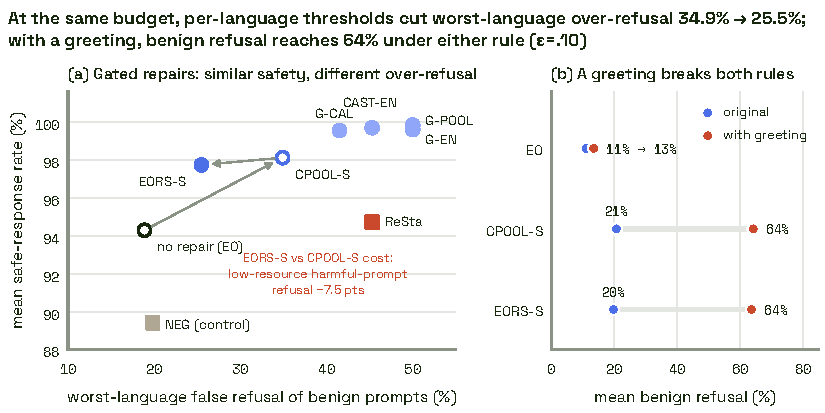
\includegraphics[width=\linewidth]{figs/fig1_teaser.pdf}
\caption{\textbf{The threshold rule sets who is over-refused; a greeting breaks every rule.} (a) Every repair arm on Tiny Aya Earth, judged by Qwen3Guard-4B on the MultiJail test split (209 harmful, 106 benign prompts per language, 10 languages): mean safe-response rate against the worst language's benign refusal rate. Arrows run from the unrepaired model (E0) to one pooled split-conformal threshold (CPOOL-S, $\varepsilon{=}.05$) and on to per-language thresholds at the same budget (EORS-S); the two share steering vector, condition direction and calibration data. Paired bootstrap intervals are in Tables~\ref{tab:arms} and~\ref{tab:controls}. (b) End-to-end greeting test ($\varepsilon{=}.10$; pre-registered secondary): mean benign refusal without and with the English prefix ``Good morning.'' in every language.}
\label{fig:teaser}
\end{figure}

\section{Related work}
\paragraph{Multilingual safety gaps.} Translating harmful requests into low-resource languages bypasses safety training~\citep{yong2023lowresource,deng2024multijail}; human-written multilingual red-teaming separates global from local harms~\citep{aakanksha2024prism}; multilingual guards such as PolyGuard~\citep{kumar2025polyguard} cover 17 languages, missing most of Tiny Aya's. Multilingual safety research remains English-dominated~\citep{yong2025state}, and judges are less accurate in lower-resource languages~\citep{zhou2026lowerresource}.
\paragraph{Refusal geometry and conditional steering.} Refusal is mediated by a low-dimensional direction~\citep{arditi2024refusal} shared across safety-aligned languages~\citep{wang2025universal}. CAST adds a refusal vector only when a condition direction fires~\citep{lee2025cast}. English-derived steering raises over-refusal in low-resource languages~\citep{stein2026babelsteering}, and their failures are \emph{action} failures: harm is represented but scores sit below the refusal range, so a per-language calibrated gate restores selectivity~\citep{aziz2026action}. \citet{aziz2026action} already run per-language calibrated conditional steering end to end, against CAST and AdaSteer~\citep{zhao2025adasteer}, and score refusal selectivity; single-vector ablation also reduces false refusal~\citep{wang2024surgical}. We build on their setting and ask what it leaves open: which threshold \emph{objective} allocates over-refusal across languages, what that allocation costs in harmful-prompt refusal and harmful answers, and how robust it is, with three-way outcomes and validated multilingual judges.
\paragraph{Safety drift and repair.} Fine-tuning erodes alignment~\citep{qi2024finetuning}, unevenly across languages~\citep{poppi2025fragility,hawkins2026heterogeneous}; ReSta restores it with a DARE-sparsified safety vector~\citep{bhardwaj2024resta}. Multilingual safety gaps are well documented~\citep{wang2023xsafety}; whether repairs close them evenly across languages has received less attention than whether they close them on average.
\paragraph{Fairness and conformal calibration.} Equal false-positive rates across groups is \emph{predictive equality}~\citep{corbettdavies2017cost}; equalised odds also equalises true-positive rates~\citep{hardt2016equality}. With group-specific thresholds each group sits at a different point of its own ROC curve, so equalising one error rate generally leaves the other unequal~\citep{hardt2016equality}; with unequal base rates, calibration and error-rate balance cannot both hold~\citep{chouldechova2017fair,kleinberg2017tradeoffs}. A conformal quantile per group is Mondrian split-conformal prediction~\citep{vovk2003mondrian,gibbs2025conditional}. Its guarantee needs a score fitted on data independent of the calibration fold and holds on average over calibration draws~\citep{angelopoulos2021gentle}; high-probability versions exist~\citep{angelopoulos2021ltt}. Detectors trained on harmful and benign sets from different sources can learn the source rather than the harm~\citep{fomin2026benchmarks,wang2025falsesense}.

\section{Setting and measurement}
\label{sec:setting}
\paragraph{Models and hardware.} Tiny Aya Global and Earth (Africa/West Asia specialisation), bf16, greedy decoding, 96 new tokens, shipped chat template, whose ``contextual safety mode'' preamble we also remove (B1). All repair arms and their paired references (E0, B0) were generated on one A100 with the same code, batch size and library versions; on E0, A100 and the original Apple-MPS generation differ by $\HwSrr$ points of mean SRR \ci{\HwSrrLo}{\HwSrrHi} with refusal-label agreement $\kappa=\HwRefKappa$, so pairs never mix hardware. On one A100 an arm takes about \ComputeGenMin{} minutes to generate all test responses and \ComputeScoreMin{} to score with Qwen3Guard-4B.
\paragraph{Data.} Harmful: MultiJail, 314 parallel prompts $\times$ 10 languages (high resource: en, zh, it, vi; medium: ar, ko, th; low: bn, sw, jv), split 105 calibration / 209 test by prompt id. Benign-but-sensitive: XSTest safe prompts~\citep{rottger2024xstest} translated with NLLB-200~\citep{costa2022nllb}, kept only where constrained GlotLID~\citep{kargaran2023glotlid} and back-translation chrF agree in \emph{all} languages (90 calibration / 106 test ids). CuratorKIT cleans, deduplicates and records provenance; ids that lose any language are dropped, so every test is fully paired. Licences: MultiJail MIT, XSTest and PolyGuardPrompts CC-BY-4.0, Aya red-teaming Apache-2.0; Tiny Aya and NLLB outputs are CC-BY-NC-4.0, which our data release inherits.
\paragraph{Outcomes.} Each response to a harmful prompt is a refusal, a safe compliance or a harmful compliance. Primary: $\SRR_\ell=1-$ harmful-compliance rate, and $\BRR_\ell$ = refusal rate on benign prompts. Behavioural: $\HRR_\ell$, refusal on harmful prompts. Fairness: worst-language SRR and worst-language BRR.
\paragraph{Judges and statistics.} Qwen3Guard-Gen-4B~\citep{qwen3guard2025} is the primary judge and Gemini~3.5 Flash (broad rubric) the second; both are validated against human labels in \S\ref{sec:measure}. Comparisons are paired by prompt id: exact McNemar tests per language with Holm correction, paired bootstrap over ids (5{,}000 resamples) for pooled estimands, Wilson intervals for rates. Each confirmatory comparison was fixed, with its reading rule, before its own outputs existed; the plan's history, including two changes of primary endpoint, is dated in Appendix~\ref{app:prereg}.

\section{Gates and arms}
\label{sec:method}
Let $h(x)\in\mathbb{R}^d$ be the residual stream at the last prompt token at layer $L$, and $v$ the unit difference of class means (harmful minus benign) over calibration prompts. A gated arm adds a steering vector $\alpha u$ to a band of layers iff a gate score exceeds a threshold at prefill.
\paragraph{CAST's score is approximately sign-invariant.} CAST~\citep{lee2025cast}, faithfully implemented in SafeTune, scores $g_{\text{CAST}}(h)=\cos\!\big(h,\tanh(v\,v^\top h)\big)$.
\begin{remark}[Sign invariance]\label{prop:cast}
Let $s=v^\top h$ with $\|v\|=1$. In the linear regime of $\tanh$ ($|s|\max_i|v_i|\ll 1$), $\tanh(sv)\approx sv$, so $g_{\text{CAST}}(h)\approx s\,v^\top h/(\|h\|\,|s|)=|s|/\|h\|$: the score ranks prompts by the magnitude of the projection, and a prompt projecting strongly \emph{negatively} scores like a strongly harmful one.
\end{remark}
The remark is a two-line identity under a linearisation. On Tiny Aya Earth's calibration activations the regime is approached for benign prompts (median $|s|\max_i|v_i|$ \CastRegimeBenMin--\CastRegimeBenMax{} across languages) but not for harmful ones (\CastRegimeHarmMin--\CastRegimeHarmMax), so it describes a tendency of the ranking, which we test empirically. Whether it matters depends on how many benign prompts project negatively, which varies by language (Appendix~\ref{app:gate}). Our own gates threshold the projection $s$ itself, and the faithful CAST gate is kept as an arm.
\paragraph{Equal-over-refusal steering (EORS).} For language $\ell$ with benign calibration scores $s^{(\ell)}_1\le\dots\le s^{(\ell)}_{n_\ell}$ and budget $\varepsilon$, set $\tau_\ell=s^{(\ell)}_{\lceil(1-\varepsilon)(n_\ell+1)\rceil}$; at inference the language comes from constrained GlotLID.
\begin{proposition}[Per-language false-firing bound]\label{prop:eors}
If the score function (layer and direction) is fitted on data independent of language $\ell$'s calibration prompts, and a new benign prompt in $\ell$ is exchangeable with them and correctly identified, then $\Pr[s>\tau_\ell]\le\varepsilon$, the probability taken over the calibration draw and the new prompt.
\end{proposition}
This is Mondrian split-conformal prediction~\citep{vovk2003mondrian}, i.e.\ predictive equality~\citep{corbettdavies2017cost} for the gate. Given one calibration set, the realised false-firing rate is itself random, $\mathrm{Beta}(n_\ell+1-k,k)$ with $k=\lceil(1-\varepsilon)(n_\ell+1)\rceil$~\citep{angelopoulos2021gentle}, and spans several points at $n_\ell\approx 60$. Our first EORS arms fitted the direction and the thresholds on the same calibration prompts, which voids the independence condition; EORS-S restores it by fitting the layer and direction on one third of the calibration ids and the thresholds on the other two thirds (\S\ref{sec:gate}). The bound concerns when the \emph{gate} fires, not the model's baseline over-refusal, and assumes exchangeability, which \S\ref{sec:brittle} stress-tests.
\paragraph{Arms (all on Tiny Aya Earth).} G-POOL: pooled steering vector and direction, one max-F1 threshold. G-EN: English vector and direction, projection gate. CAST-EN: as G-EN with CAST's gate score. G-CAL: per-language max-F1 thresholds (after~\citealp{aziz2026action}). EORS at $\varepsilon\in\{.05,.10\}$ (thresholds fitted in-sample). EORS-S: EORS with the split fit above. CPOOL-S, the matched-budget control: the same split, direction and $\varepsilon$, with one conformal threshold on the pooled benign scores of all languages (a marginal guarantee only). ReSta: SafeTune's \texttt{apply\_resta} ($\alpha{=}0.25$, DARE $p{=}0.3$). NEG: the steering vector negated (control). Steering strength was fixed before any arm ran by a rule on calibration data only (largest $\alpha$ keeping responses on-language and non-degenerate): $\alpha=\AlphaPick$, where ungated steering already refuses \AlphaOneHrr{} of harmful and \AlphaOneBrr{} of benign calibration prompts, so the gate carries all selectivity; at $\alpha=2$ only \AlphaTwoOnLang{} of responses stay on-language.

\section{Results}
\label{sec:results}

\subsection{The threshold rule allocates over-refusal and protection (pre-registered)}
\label{sec:gate}
\begin{table}[t]
\caption{\textbf{Every gated arm buys a similar safety gain; arms differ in over-refusal.} Paired change against the unrepaired model (E0, Tiny Aya Earth; B1 against B0, Tiny Aya Global), percentage points, Qwen3Guard-4B, 95\% paired bootstrap intervals over prompt ids; point estimates are the statistic on the observed data. Worst-language BRR is the maximum over the ten languages. EORS rows use thresholds fitted on the same prompts as the direction (superseded by EORS-S, Table~\ref{tab:controls}).}
\label{tab:arms}
\centering\resizebox{\linewidth}{!}{% AUTO-GENERATED by src/refusal_parity/reporting/paper_numbers/ from runs/arms_report.json (q3g4b)
\begin{tabular}{@{}llccc@{}}
\toprule
Arm & Gate / change & $\Delta$ mean SRR & $\Delta$ worst-language BRR & $\Delta$ mean HRR \\
\midrule
G-POOL & single pooled threshold & $+5.3$ {\scriptsize[$+3.8$, $+7.0$]} & $+31.1$ {\scriptsize[$+22.6$, $+40.6$]} & $+33.2$ {\scriptsize[$+28.7$, $+37.6$]} \\
G-EN & English vector, projection gate & $+5.6$ {\scriptsize[$+4.0$, $+7.3$]} & $+31.1$ {\scriptsize[$+23.6$, $+41.5$]} & $+36.1$ {\scriptsize[$+31.5$, $+40.7$]} \\
CAST-EN & English vector, CAST gate & $+5.4$ {\scriptsize[$+3.9$, $+7.1$]} & $+26.4$ {\scriptsize[$+18.9$, $+34.9$]} & $+34.1$ {\scriptsize[$+29.7$, $+38.6$]} \\
G-CAL & per-language max-F1 & $+5.3$ {\scriptsize[$+3.8$, $+6.9$]} & $+22.6$ {\scriptsize[$+16.0$, $+32.1$]} & $+33.2$ {\scriptsize[$+28.7$, $+37.7$]} \\
EORS $\varepsilon{=}.10$ & per-language conformal & $+5.1$ {\scriptsize[$+3.6$, $+6.8$]} & $+11.3$ {\scriptsize[$+5.7$, $+17.9$]} & $+31.1$ {\scriptsize[$+26.7$, $+35.6$]} \\
EORS $\varepsilon{=}.05$ & per-language conformal & $+4.5$ {\scriptsize[$+3.1$, $+6.0$]} & $+6.6$ {\scriptsize[$+0.9$, $+11.3$]} & $+24.9$ {\scriptsize[$+21.1$, $+29.0$]} \\
ReSta & weight arithmetic & $+0.4$ {\scriptsize[$-1.0$, $+1.9$]} & $+26.4$ {\scriptsize[$+17.0$, $+34.9$]} & $+8.3$ {\scriptsize[$+6.2$, $+10.5$]} \\
NEG & negative control & $-4.9$ {\scriptsize[$-6.2$, $-3.6$]} & $+0.9$ {\scriptsize[$-4.7$, $+8.5$]} & $-3.6$ {\scriptsize[$-5.8$, $-1.5$]} \\
\midrule
B1 (no preamble) & vs.\ B0, Tiny Aya Global & $+0.0$ {\scriptsize[$-0.6$, $+0.7$]} & $+3.8$ {\scriptsize[$-2.8$, $+10.4$]} & $+1.5$ {\scriptsize[$+0.3$, $+2.8$]} \\
\bottomrule
\end{tabular}
}
\end{table}
The gated arms of Table~\ref{tab:arms} raise mean SRR by \ArmsQSrrGainMin{} to \ArmsQSrrGainMax{} points over E0, and the split arms of Table~\ref{tab:controls} by \CtlSrrGainMin{} to \CtlSrrGainMax. E0 is already at \EZeroAhundredSrr, so this gain is near the ceiling and does not discriminate between arms. Over-refusal does: arms with a single threshold or per-language max-F1 thresholds raise worst-language BRR by \ArmsQMaxBrrMin{} to \ArmsQMaxBrrMax{} points.

\paragraph{The first contrast mixed level with spread.} Our pre-registered contrast held the steering vector and direction fixed and replaced G-POOL's single max-F1 threshold with per-language conformal thresholds (EORS). Worst-language BRR fell by $\EorsQMaxBrr$ points \ci{\EorsQMaxBrrLo}{\EorsQMaxBrrHi}, but mean BRR fell too ($\EorsQMeanBrr$), and the worst $\div$ mean ratio did not move (\GpoolBrrRatio{} vs.\ \EorsBrrRatio): EORS was mostly a stricter rule, not a fairer one. Its direction and thresholds were also fitted on the same calibration prompts, which voids Prop.~\ref{prop:eors}. Both points came from independent reviews of an earlier draft.

\paragraph{Matched-budget control (pre-registered).} We therefore compared EORS-S with CPOOL-S, which share steering vector, condition direction, calibration fold and budget $\varepsilon$ and differ only in whether the conformal threshold is set per language or pooled (Table~\ref{tab:controls}, Fig.~\ref{fig:eors}). The co-primary estimands and their reading rules were fixed before generation; Holm correction runs over the two budgets.
At $\varepsilon{=}.05$, per-language thresholds lower worst-language BRR by $\CtlFiveMaxBrr$ points \ci{\CtlFiveMaxBrrLo}{\CtlFiveMaxBrrHi} (\CtlFivePoneHolm), from \CtlFivePoolWorstBrr{} to \CtlFiveEorsWorstBrr{} in \CtlFivePoolWorstBrrLang, while mean BRR does not rise ($\CtlFiveMeanBrr$ \ci{\CtlFiveMeanBrrLo}{\CtlFiveMeanBrrHi}); the worst $\div$ mean ratio falls from \CtlFivePoolRatio{} to \CtlFiveEorsRatio, the cross-language range by $\CtlFiveRange$ \ci{\CtlFiveRangeLo}{\CtlFiveRangeHi}, and no language's benign refusal exceeds E0's by more than \CtlFiveEorsExcessMax{} points (single threshold: \CtlFivePoolExcessMax). \CtlFivePoolWorstBrrLang{} is the worst language under both rules and the only one whose benign change survives per-language Holm correction (\CtlTenHolmBenignLangs{} at $\varepsilon{=}.10$); the reported $p$ is the bootstrap floor for this max-type statistic. At $\varepsilon{=}.10$ the result is the same ($\CtlTenMaxBrr$ \ci{\CtlTenMaxBrrLo}{\CtlTenMaxBrrHi}, \CtlTenPoneHolm).
The price lands on the languages whose benign prompts score highest, which pull their thresholds up: harmful-prompt refusal falls in \CtlFiveHrrLossLang{} ($\CtlFiveHrrLossPts$), Bengali ($\CtlFiveHrrBn$) and Thai ($\CtlFiveHrrTh$), not in Swahili ($\CtlFiveHrrSw$), and rises in high-resource languages (\CtlFiveHrrGainLang{} $\CtlFiveHrrGainPts$). In the pre-registered low-resource tier it falls by $\CtlFiveLrlHrr$ points \ci{\CtlFiveLrlHrrLo}{\CtlFiveLrlHrrHi} (\CtlFivePtwoHolm; $\varepsilon{=}.10$: $\CtlTenLrlHrr$). The cross-language range of harmful-prompt refusal barely moves (\CtlFivePoolHrrRange{} vs.\ \CtlFiveEorsHrrRange{} points), but the gap between the high- and low-resource tiers grows from \CtlFivePoolTierGap{} to \CtlFiveEorsTierGap{} points. Harmful answers in that tier rise by $\CtlFiveLrlUnsafe$ points \ci{\CtlFiveLrlUnsafeLo}{\CtlFiveLrlUnsafeHi} at $\varepsilon{=}.05$ and $\CtlTenLrlUnsafe$ \ci{\CtlTenLrlUnsafeLo}{\CtlTenLrlUnsafeHi} at $.10$; mean SRR changes by $\CtlFiveSrr$.
Group-specific thresholds that equalise one error rate place each group at a different point of its own ROC curve, so the other error rate generally differs~\citep{hardt2016equality}; which languages lose is empirical, and here it is those whose benign prompts score high, as the calibration-only design check predicted. Per-language calibration makes over-refusal more equal and protection less equal between tiers. Which error to equalise is a policy choice; Appendix Fig.~\ref{fig:frontier} gives the gate-level frontier across budgets.

\paragraph{The per-language bound is not contradicted, and the trade-off survives redrawing the split.} On held-out benign prompts (gate level), EORS-S's false-firing is \CtlFiveValidMeanFpr{} on average at $\varepsilon{=}.05$ and stays inside its predictive band in every language at both budgets, whether thresholds are routed by the true or the detected language (pre-registered); the in-sample EORS thresholds reached up to \CtlFiveInsampleMaxFpr. With $n_\ell=\CtlNCal$ calibration prompts the band is wide (97.5th percentile \CtlFiveBand{} at $\varepsilon{=}.05$, \CtlTenBand{} at $.10$), and the pre-registration fixed a single fit/conformal split. Redrawing that split \CtlSplitN{} times (exploratory), at most \CtlSplitAboveMax{} language exceeds the band (none in \CtlSplitAboveZero{} of draws); per-language thresholds lower worst-language false-firing in \CtlSplitDMaxShare{} of draws (median $\CtlSplitDMax$ points, 95\% of draws in [$\CtlSplitDMaxLo$, $\CtlSplitDMaxHi$]) and low-resource detection in \CtlSplitDLrlShare{} (median $\CtlSplitDLrl$); their mean false-firing is also slightly lower in \CtlSplitMeanLowerShare{} of draws (median $\CtlSplitDMean$), far less than the worst-language change. Post hoc, realised rates within a draw move together across languages because the prompt ids are parallel, and at budgets of \CtlFrontExceedEps{} and above \CtlFrontExceedMin--\CtlFrontExceedMax{} languages exceed the band in the frontier, so the bound should be read as holding on average over calibration draws, not for each. Recomputing the calibration activations on the A100 shows that hardware and batching shift gate scores by a standard deviation of only \CtlHwSd{} and \CtlBatchSd{} (score s.d.\ \CtlScoreSd), so prompt sampling, not the hardware pairing, explains the gap between calibration and test score distributions.

The in-sample EORS contrast also holds at half the steering strength ($\alpha{=}0.5$; $\AhEorsMaxBrr$ points; Appendix Table~\ref{tab:arms05}); since gate thresholds do not depend on $\alpha$, this is a robustness check on the steering strength, not an independent replication.

\begin{table}[t]
\caption{\textbf{Matched-budget controls} (pre-registered 2026-10-28; Tiny Aya Earth, A100, $\alpha{=}1$, Qwen3Guard-4B). Top: each arm against the unrepaired model. Bottom: per-language against pooled split-conformal thresholds at the same budget, the pre-registered contrast. Percentage points, 95\% paired bootstrap intervals over prompt ids; low-resource tier: bn, sw, jv.}
\label{tab:controls}
\centering\resizebox{\linewidth}{!}{% AUTO-GENERATED by src/refusal_parity/reporting/paper_numbers/ from runs/arms_report.json (q3g4b)
\begin{tabular}{@{}llcccc@{}}
\toprule
Arm & Reference & $\Delta$ mean SRR & $\Delta$ worst-language BRR & $\Delta$ mean BRR & $\Delta$ HRR, low-resource tier \\
\midrule
CPOOL-S $\varepsilon{=}.05$ & vs.\ E0 & $+3.8$ {\scriptsize[$+2.6$, $+5.2$]} & $+16.0$ {\scriptsize[$+8.5$, $+22.6$]} & $+4.5$ {\scriptsize[$+2.6$, $+6.7$]} & $+29.5$ {\scriptsize[$+24.6$, $+34.4$]} \\
EORS-S $\varepsilon{=}.05$ & vs.\ E0 & $+3.4$ {\scriptsize[$+2.2$, $+4.7$]} & $+6.6$ {\scriptsize[$+1.9$, $+11.3$]} & $+3.5$ {\scriptsize[$+1.6$, $+5.9$]} & $+22.0$ {\scriptsize[$+17.5$, $+26.6$]} \\
CPOOL-S $\varepsilon{=}.10$ & vs.\ E0 & $+4.3$ {\scriptsize[$+3.0$, $+5.7$]} & $+24.5$ {\scriptsize[$+16.0$, $+32.1$]} & $+9.6$ {\scriptsize[$+6.5$, $+13.0$]} & $+35.7$ {\scriptsize[$+30.6$, $+41.0$]} \\
EORS-S $\varepsilon{=}.10$ & vs.\ E0 & $+4.5$ {\scriptsize[$+3.1$, $+6.1$]} & $+16.0$ {\scriptsize[$+8.5$, $+22.6$]} & $+8.7$ {\scriptsize[$+5.5$, $+12.4$]} & $+28.4$ {\scriptsize[$+23.6$, $+33.2$]} \\
\midrule
EORS-S $\varepsilon{=}.05$ & vs.\ CPOOL-S & $-0.4$ {\scriptsize[$-0.8$, $-0.0$]} & $-9.4$ {\scriptsize[$-15.1$, $-3.8$]} & $-1.0$ {\scriptsize[$-2.2$, $+0.0$]} & $-7.5$ {\scriptsize[$-9.6$, $-5.4$]} \\
EORS-S $\varepsilon{=}.10$ & vs.\ CPOOL-S & $+0.2$ {\scriptsize[$-0.1$, $+0.6$]} & $-8.5$ {\scriptsize[$-14.2$, $-3.8$]} & $-0.9$ {\scriptsize[$-2.4$, $+0.4$]} & $-7.3$ {\scriptsize[$-9.4$, $-5.3$]} \\
\bottomrule
\end{tabular}
}
\end{table}

\begin{figure}[t]
\centering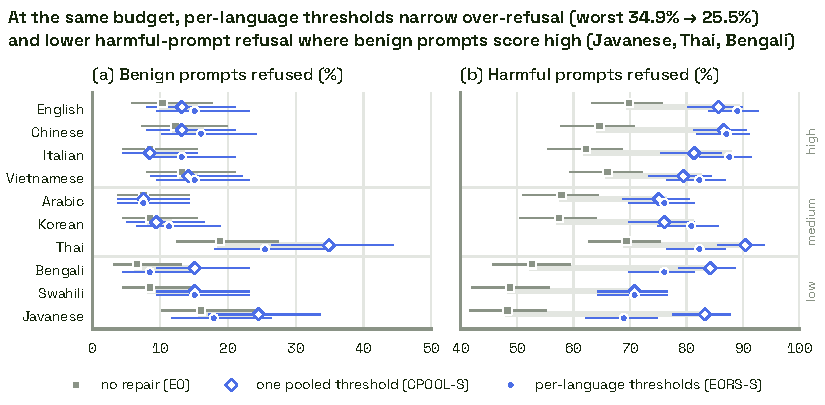
\includegraphics[width=\linewidth]{figs/fig2_eors.pdf}
\caption{\textbf{Same steering, same budget, different threshold rule.} Tiny Aya Earth, $\alpha{=}1$, $\varepsilon{=}.05$. CPOOL-S and EORS-S share steering vector, condition direction, calibration fold and false-refusal budget and differ only in whether the split-conformal threshold is pooled over languages or set per language; E0 is unrepaired. Qwen3Guard-4B labels; 95\% Wilson intervals; languages grouped by resource tier. Paired tests are in Table~\ref{tab:controls}.}
\label{fig:eors}
\end{figure}

\subsection{CAST's gate score is approximately sign-invariant; its end-to-end cost is not separable (H6, exploratory status)}
\label{sec:cast}
At the gate level, on Tiny Aya Global's held-out activations, CAST loses separability in proportion to the share of benign prompts projecting negatively (Pearson $r=\CastPearson$ across languages; Swahili AUROC \CastAurocSwProj{}$\rightarrow$\CastAurocSwCast; Appendix~\ref{app:gate}), the regime Remark~\ref{prop:cast} identifies.
End to end, we compare CAST-EN with G-EN, which share the English steering vector and condition direction and differ only in the gate score (Appendix Fig.~\ref{fig:cast}).
The pre-registered primary estimate supports the predicted direction: in the low-resource tier CAST-EN refuses $\CastQLrlHrr$ points fewer harmful prompts \ci{\CastQLrlHrrLo}{\CastQLrlHrrHi} (Gemini $\CastGLrlHrr$ \ci{\CastGLrlHrrLo}{\CastGLrlHrrHi}), and it refuses fewer in \CastNNeg{} of 10 languages.
Two qualifications matter. The effect does not reach harmful answers ($\CastQLrlUnsafe$ points), because at $\alpha=\AlphaPick$ both gates refuse almost all harmful prompts; and across languages the loss does not track the negative-projection share (Spearman $\rho=\CastRho$), so the gate-level mechanism does not carry over cleanly to behaviour. No single language survives Holm correction (\CastNSig{} of 10): with \CastPowerPsi{} of pairs discordant, \CastPowerMde{} at $\alpha=0.05$.
CAST-EN also over-refuses less: worst-language BRR changes by $\CastQMaxBrr$ points \ci{\CastQMaxBrrLo}{\CastQMaxBrrHi}, mean BRR by $\CastQMeanBrr$, and benign refusal falls after Holm correction in \CastNSigBrr{} languages. Lower refusal on both prompt types with unchanged SRR is what a stricter operating point produces, and CAST's threshold is chosen by max-F1 on English in a different score space; the end-to-end contrast therefore does not isolate the sign invariance from an operating-point shift.
We pre-registered the prediction that the effect grows when steering is weaker. At $\alpha{=}0.5$ the test is indeterminate: both gated arms are at ceiling (Appendix Table~\ref{tab:arms05}), the low-resource estimate ($\AhCastLrlHrr$ points \ci{\AhCastLrlHrrLo}{\AhCastLrlHrrHi}) is close to $\alpha{=}1$'s, and we fixed no interval for the difference.
We read the sign invariance as a property of the score worth fixing in CAST-style gates; whether it costs behaviour on this model is unresolved.


\subsection{Measurement decides what is seen (H1 pre-registered; judge validation)}
\label{sec:measure}
SafeTune ships two English keyword refusal detectors, which the Lexsi stack uses to score refusal and choose steering layers. On all B0 responses they agree with Qwen3Guard in English ($\kappa=\HOneKappaEnMin$--\HOneKappaEnMax) and detect \HOneRecallOtherMax{} of refusals in each of the nine other languages (Fig.~\ref{fig:instruments}a); the pre-registered English-vs-rest agreement gap is \HOneGap{} \ci{\HOneGapLo}{\HOneGapHi}. A keyword audit would report that the model never refuses outside English.
Against \NValidation{} human-labelled PolyGuardPrompts items in seven languages, both judges detect refusal well ($\kappa=\QRefKappaMean$ Qwen3Guard, \RefKappaMean{} Gemini), but on harm Qwen3Guard reaches $\kappa=\QHarmKappaMean$ and Gemini only \HarmKappaMean, missing \QHarmMiss{} and \GemHarmMiss{} of harmful responses (Fig.~\ref{fig:instruments}b). Misses concentrate where annotators split 2--1 (Qwen3Guard \QHarmMissSplit, vs.\ \QHarmMissUnanimous{} on unanimous items).
Refusal is not safety: a closed model, Gemini~3.5 Flash-Lite, refuses only \GemHRRMin--\GemHRRMax{} of MultiJail prompts and its responses are \GemGSrr{} safe under the Gemini judge but \GemQSrr{} under Qwen3Guard, close to the unrepaired Tiny Aya Earth's \EZeroAhundredSrr. The Gemini judge is lenient in general (harm $\kappa=\HarmKappaMean$), but more so on its own family's outputs: its unsafe-rate gap to Qwen3Guard is \CtlJudgeGapGem{} points on Gemini's responses and \CtlJudgeGapEZero{} on Tiny Aya's, a difference of $\CtlJudgeDid$ \ci{\CtlJudgeDidLo}{\CtlJudgeDidHi} (post hoc), consistent with LLM judges favouring their own generations~\citep{panickssery2024selfpref,zheng2023judging}. We therefore treat harmful compliance as the safety outcome and refusal as behaviour, and report harm under both judges.

\begin{figure}[t]
\centering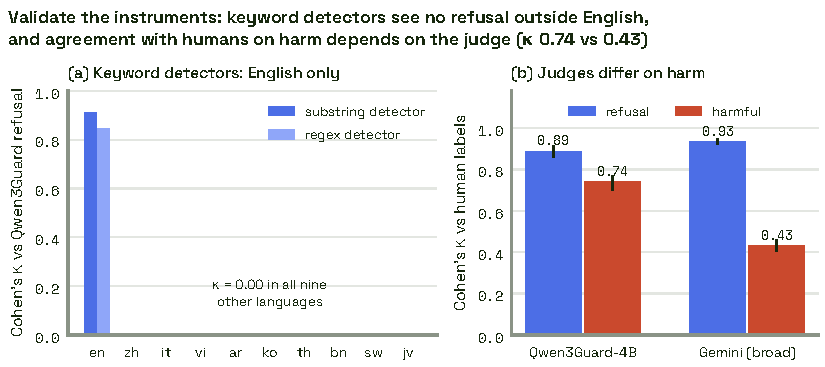
\includegraphics[width=\linewidth]{figs/fig4_instruments.pdf}
\caption{\textbf{Instrument validity.} (a) Agreement between SafeTune's English keyword refusal detectors and Qwen3Guard-4B refusal labels on all B0 responses (Tiny Aya Global), per language (H1). (b) Agreement of each judge with PolyGuardPrompts human labels on \NValidation{} items in en, hi, it, th, zh, ar, ko; bars: mean over languages, whiskers: range. None of our low-resource languages is among the validation languages.}
\label{fig:instruments}
\end{figure}

\subsection{Gate calibration on clean prompts does not survive a greeting (found post hoc; tested end to end)}
\label{sec:brittle}
EORS picks its threshold from the detected language, so we tested whether adding text in another language lets an attacker route a harmful prompt to a laxer threshold. It does not: an English prefix flips language identification for up to \BritLidFlipMax{} of harmful prompts, but the gate fires \emph{more} on prefixed harmful prompts, not less.
The same experiment exposed a larger problem on benign prompts (Fig.~\ref{fig:teaser}b; Appendix Fig.~\ref{fig:brittle}). Gate false-firing averages \BritOrigMean{} on the original prompts and rises to \BritEnMean{} with an English instruction prefix, \BritNativeMean{} with the same instruction in the prompt's own language, and \BritGreetMean{} with ``Good morning.'' Language identification is unchanged for the own-language and greeting prefixes, and among benign prompts the gate score is unrelated to prompt length, so neither code-mixing nor length explains the shift. We leave the mechanism open.

\paragraph{End-to-end test (pre-registered).} We then tested the finding end to end with an analysis fixed before generation, on the same test prompts on which it was found and with the most disruptive prefix of the control set: EORS ($\varepsilon{=}.10$, in-sample thresholds) and the unrepaired model, each with every prompt prefixed by ``Good morning.'', and with the gate's language detected on the prefixed prompt, as at inference; the English greeting is used in every language, and labels are Qwen3Guard-only. The estimand is a difference-in-differences in benign refusal, the repair's added refusal with the greeting minus its added refusal without it, which removes the greeting's effect on the model itself. It is $\GreetDid$ points \ci{\GreetDidLo}{\GreetDidHi}, with an interval above zero in all \GreetDidNPos{} languages (\GreetDidLangMin{} to \GreetDidLangMax{}), English included. The greeting barely moves the unrepaired model (\GreetBrrEZero{} to \GreetBrrEZeroGreet{} benign refusal) but takes the repaired one from \GreetBrrEors{} to \GreetBrrEorsGreet. Harmful answers do not change (difference-in-differences $\GreetDidUnsafe$ points \ci{\GreetDidUnsafeLo}{\GreetDidUnsafeHi}): the greeting does not unlock harm; it makes the repair refuse ordinary questions.

\paragraph{Both threshold rules break (pre-registered secondary).} With the controls we repeated the test for EORS-S and CPOOL-S ($\varepsilon{=}.10$). The difference-in-differences in benign refusal is $\CtlGreetDidEors$ points \ci{\CtlGreetDidEorsLo}{\CtlGreetDidEorsHi} for per-language thresholds and $\CtlGreetDidPool$ \ci{\CtlGreetDidPoolLo}{\CtlGreetDidPoolHi} for the pooled one: mean benign refusal rises from \CtlGreetBrrEors{} to \CtlGreetBrrEorsGreet{} and from \CtlGreetBrrPool{} to \CtlGreetBrrPoolGreet. Per-language thresholds still cap the worst language lower (\CtlGreetWorstEors{} vs.\ \CtlGreetWorstPool), but the brittleness belongs to the gate's direction and calibration distribution, not to its threshold rule.

\paragraph{The gate detects harm, not only the benchmark's style.} Harmful (MultiJail) and benign (XSTest) prompts come from different sources, so the direction could encode provenance~\citep{fomin2026benchmarks,wang2025falsesense}. On XSTest's own unsafe contrast prompts, which share the benign prompts' surface form (\CtlXsN{} ids, translated with the same pipeline), the gate score separates unsafe from safe with AUROC \CtlStyleAuc{} pooled and at least \CtlStyleAucMin{} in every language (pre-registered rule: harm signal beyond style), against \CtlMjAuc{} for MultiJail. XSTest's unsafe prompts are minimal pairs, harder by design, so the gap does not measure how much of MultiJail's separability is style. On unseen harmful prompts from Aya red-teaming the gate fires on \CtlOodEn{} (English) and \CtlOodAr{} (Arabic) at $\varepsilon{=}.05$, against \CtlMjFireEn{} and \CtlMjFireAr{} of MultiJail's harmful test prompts; in the six Aya languages outside our ten, which fall back to the strictest threshold, it fires on \CtlOodOtherMin--\CtlOodOtherMax.

The practical consequence is that the conformal guarantee (Prop.~\ref{prop:eors}) holds for prompts exchangeable with the calibration set, and ordinary conversational framing breaks exchangeability. Any gate calibrated on benchmark prompts should be re-calibrated on, or at least tested against, the formats users actually send.

\subsection{Secondary results}
\label{sec:secondary}
\paragraph{Natural drift (pre-registered).} On identical prompts Tiny Aya Earth is slightly less safe than Global: mean SRR $\DriftQSrr$ points \ci{\DriftQSrrLo}{\DriftQSrrHi} under Qwen3Guard and $\DriftGSrr$ under Gemini, with no language significant after Holm correction (Appendix~\ref{app:drift}). Power, not the model, sets this limit: only \PowerPsiHarm{} of paired prompts change label, so a per-language test reaches 80\% power~\citep{connor1987mcnemar} only for effects of \PowerMdeHarm{} at $\alpha{=}0.05$, and none after Holm correction. The Tiny Aya report finds a larger worst-language loss (\ReportMinSafeGlobal{} to \ReportMinSafeEarth{} with a different judge and the full set;~\citealp{salamanca2026tinyaya}); we read our estimate as drift under this protocol, not a contradiction.
\paragraph{Detection survives drift (H3).} In the languages with the largest drift, harm-direction AUROC drops by at most \HThreeAurocDropMax{} (pre-registered threshold 0.03), so drift is not a detection failure; a scale-free margin does not single out those languages either (post hoc), so we claim no language-specific action failure.
\paragraph{The preamble does not carry safety.} Removing the chat template's safety preamble (B1) changes mean SRR by $\PreQSrr$ points \ci{\PreQSrrLo}{\PreQSrrHi} and harmful-prompt refusal by $\PreQHrr$: at this near-ceiling safety level the preamble carries no measurable safety.
\paragraph{Weight-space repair does not help here.} ReSta changes mean SRR by $\RestaQSrr$ points \ci{\RestaQSrrLo}{\RestaQSrrHi} while raising worst-language BRR by $\RestaQMaxBrr$. The NEG control changes SRR by $\NegQSrr$ points, as a sign-flipped vector should.
\paragraph{Cost.} The closed comparator cost \RoiGemCost{} for \RoiGemN{} responses at list price; Tiny Aya has no per-token fee and generated \RoiTinyPerMin{} responses per minute on a 16\,GB laptop. Self-hosting removes the per-token cost; it does not remove the need to audit a repair in every language.

\section{Discussion and limitations}
\label{sec:limitations}
\paragraph{What generalises, and what may not.} Once steering is strong enough to refuse reliably, a gated repair is a classifier followed by a forced refusal, and its fairness is a property of the classifier's threshold rule and calibration data. Three lessons follow from the structure of that problem rather than from this model: per-group calibration of scores whose distributions differ moves protection between groups; a calibration set of parallel translations makes per-group errors move together (a post hoc observation); and calibration on benchmark-formatted prompts does not cover conversational framing. The magnitudes are for one 3B model family at one steering strength (with a robustness check at a second) and one translation pipeline.
\paragraph{Recommendations.} Report per-language false-refusal \emph{and} harmful-prompt refusal for any gated repair, at matched budgets; fit the gate direction and the thresholds on disjoint data; calibrate on, or test against, the formats users send; and check a closed model with a judge outside its family.
\paragraph{Limitations.} (i) One model family, ten languages, MultiJail and machine-translated XSTest prompts; benign probes are translated, not native. (ii) Judges are validated against humans in seven languages that include none of our low-resource tier; harm metrics are reported under both judges, and the controls and follow-ups under Qwen3Guard only. (iii) Greedy decoding and $\alpha{=}1$ (robustness check at $0.5$). (iv) The controls reuse the test prompts of the earlier contrasts with new estimands; only the XSTest-unsafe and Aya red-teaming sets are unseen. The pre-registered contrast rests on one fit/conformal split (redrawn only at gate level) and its worst language is Thai under both rules; Remark~\ref{prop:cast}'s linear regime holds only approximately. (v) With $\CtlNCal$ calibration prompts per language the per-language bound is loose, and we give no high-probability (PAC) version, which would need far more calibration data~\citep{angelopoulos2021ltt}. (vi) Per-language effects of a few points are below this design's power; pooled tier estimates are what it resolves. (vii) Not run: the strict-preamble arm, generation-level adaptive attacks, capability benchmarks, and a second model family.

\section*{AI use disclosure}
Implementation and drafting were a collaboration between the author and an AI agent (Claude, Anthropic, via Claude Code), as a reference build for the Lexsi AI Safety \& Alignment Hackathon; the author acknowledges this contribution. Procedures from the Scientific Agent Skills library~\citep{kassis2026skills} (peer review, scientific writing, visualisation, citation checks) were used, and two independent AI reviewer agents critiqued a previous draft; the controls in \S\ref{sec:gate} answer their main findings. All numbers are generated from result files by script.

\section*{Broader impact and ethics}
The work aims to make safety repair accountable to speakers of low-resource languages. Harmful prompts come from public benchmarks; we release judgments and aggregate statistics, not new attack content. Steering artefacts can be inverted to remove refusal; we will release them only under gated access with this caveat, as we will model responses. The brittleness result is a reason to test gates against realistic inputs before deployment, not an attack recipe.

\bibliographystyle{plainnat}
\bibliography{refs}

\appendix
\section{Pre-registration and deviations}
\label{app:prereg}
The analysis plan (\url{research/00_research_plan.md}) was written before any model output and amended with dated entries as the study progressed. It is an internal, timestamped log kept by the same agent that ran the analysis, not an external registry, and its primary endpoints changed twice. The original H5 (2026-10-26) required EORS to narrow the cross-language SRR gap and to keep every language's BRR within E0${}+\varepsilon$ at a capability cost of at most one point; the plan of 2026-10-27 18:50 made worst-language BRR against G-POOL primary, after the post hoc gate-level analyses. By the original H5, EORS ($\varepsilon{=}.05$) fails: the SRR gap widens by $\EorsQGapSrr$ points \ci{\EorsQGapSrrLo}{\EorsQGapSrrHi}, benign refusal exceeds E0 by more than five points in \EorsExcessNAbove{} languages (most in \EorsExcessMaxLang, $+\EorsExcessMax$), and capability was not measured. Deviations that affect this paper: steering strength chosen by a calibration-only rule fixed before the sweep; the end-to-end comparisons fixed before any steering result was inspected; G-EN added as the comparator H6 names; generation moved to an A100 with same-hardware references after a hardware-agreement check; the brittleness controls and the CircuitKIT faithfulness redesign are post hoc and labelled as such. After the $\alpha{=}1$ results, two follow-ups were pre-registered with their reading rules before generation (deviations log, 2026-10-27 23:45): the $\alpha{=}0.5$ robustness check (Table~\ref{tab:arms05}) and the end-to-end greeting test (\S\ref{sec:brittle}); both are scored by Qwen3Guard-4B only. After two independent AI reviews of the resulting draft, the matched-budget controls were pre-registered with research notes and a premortem (deviations log, 2026-10-28 06:40; \url{research/11_controls_premortem.md}): EORS-S and CPOOL-S at two budgets, two co-primary estimands with Holm correction, a gate-level validity check and a harm-versus-style check, all read by rules fixed before generation. A seed clarification was logged before any control result existed. The hardware and batching diagnostic, the correlated-error reading, the closed model's re-scoring with Qwen3Guard and the judge-gap difference-in-differences are post hoc; redrawing the calibration split and the frontier are exploratory. An independent re-review of the revised draft prompted the tier-gap reporting, routing the validity check through language identification, and the split redraws.

\begin{table}[!htbp]
\caption{\textbf{Replication at half the steering strength} ($\alpha{=}0.5$, Tiny Aya Earth, A100, Qwen3Guard-4B). Paired changes in percentage points, 95\% paired bootstrap intervals over prompt ids; the top block is against the unrepaired model (E0), the bottom block repeats the two pre-registered contrasts.}
\label{tab:arms05}
\centering\resizebox{\linewidth}{!}{% AUTO-GENERATED by src/refusal_parity/reporting/paper_numbers/ from runs/arms_report.json (q3g4b)
\begin{tabular}{@{}llccc@{}}
\toprule
Arm & Reference & $\Delta$ mean SRR & $\Delta$ worst-language BRR & $\Delta$ mean HRR \\
\midrule
G-POOL & vs.\ E0 & $+5.3$ {\scriptsize[$+3.8$, $+7.0$]} & $+21.7$ {\scriptsize[$+16.0$, $+30.2$]} & $+26.3$ {\scriptsize[$+22.8$, $+29.9$]} \\
EORS $\varepsilon{=}.05$ & vs.\ E0 & $+4.4$ {\scriptsize[$+3.1$, $+6.0$]} & $+3.8$ {\scriptsize[$+0.0$, $+7.5$]} & $+19.5$ {\scriptsize[$+16.4$, $+22.8$]} \\
G-EN & vs.\ E0 & $+5.6$ {\scriptsize[$+4.1$, $+7.4$]} & $+28.3$ {\scriptsize[$+19.8$, $+37.7$]} & $+31.9$ {\scriptsize[$+27.8$, $+36.0$]} \\
CAST-EN & vs.\ E0 & $+5.5$ {\scriptsize[$+4.0$, $+7.2$]} & $+22.6$ {\scriptsize[$+15.1$, $+31.1$]} & $+30.0$ {\scriptsize[$+26.1$, $+34.1$]} \\
\midrule
EORS $\varepsilon{=}.05$ & vs.\ G-POOL & $-0.9$ {\scriptsize[$-1.3$, $-0.4$]} & $-17.9$ {\scriptsize[$-27.4$, $-12.3$]} & $-6.8$ {\scriptsize[$-8.3$, $-5.4$]} \\
CAST-EN & vs.\ G-EN & $-0.1$ {\scriptsize[$-0.4$, $+0.0$]} & $-5.7$ {\scriptsize[$-11.3$, $+0.0$]} & $-1.9$ {\scriptsize[$-3.0$, $-1.0$]} \\
\bottomrule
\end{tabular}
}
\end{table}

\section{Gate-level analyses}
\label{app:gate}
This appendix holds the gate-level evidence behind \S\ref{sec:gate} and \S\ref{sec:brittle}: CAST against the projection gate, end to end (Figure~\ref{fig:cast}) and on held-out activations (Figure~\ref{fig:castgate}); the pooled and per-language threshold frontier (Figure~\ref{fig:frontier}); gate parity and harm detection on Tiny Aya Global (Figures~\ref{fig:gates} and~\ref{fig:mech}); prefix brittleness (Figure~\ref{fig:brittle}); and Table~\ref{tab:arms} under the second judge (Table~\ref{tab:arms-gem}).
\begin{figure}[!htbp]
\centering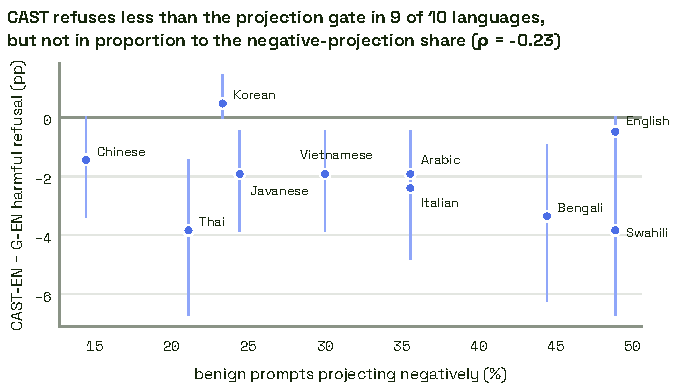
\includegraphics[width=0.82\linewidth]{figs/fig3_cast_end_to_end.pdf}
\caption{\textbf{CAST vs.\ the projection gate, end to end.} Paired per-language change in harmful-prompt refusal, CAST-EN minus G-EN (Tiny Aya Earth, Qwen3Guard-4B), against the share of benign calibration prompts projecting negatively on the condition vector (the quantity Remark~\ref{prop:cast} links to CAST's loss). Bars: 95\% bootstrap over prompt ids.}
\label{fig:cast}
\end{figure}
\begin{figure}[!htbp]
\centering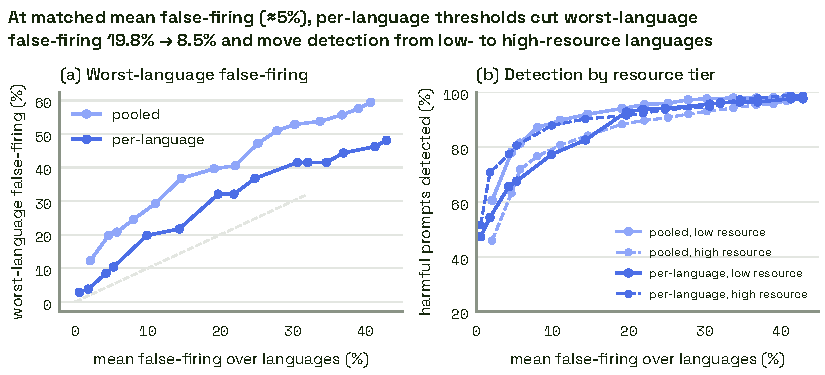
\includegraphics[width=\linewidth]{figs/figA_frontier.pdf}
\caption{Gate-level frontier on Tiny Aya Earth's test activations (EORS-S direction, layer 13). For budgets $\varepsilon=.02$ to $.30$, thresholds from the conformal fold, pooled or per language: realised mean and worst-language false-firing on benign test prompts (a), and mean detection of harmful test prompts in the low- and high-resource tiers (b). At matched mean false-firing (\CtlFrontMatchMeanPool{} pooled, \CtlFrontMatchMeanMond{} per-language), per-language thresholds cut worst-language false-firing from \CtlFrontMatchMaxPool{} to \CtlFrontMatchMaxMond. At similar mean false-firing ($\varepsilon{=}.10$: \CtlFrontMeanFprTenMond{} vs.\ \CtlFrontMeanFprTenPool), they detect \CtlFrontLrlTprTenMond{} of low-resource harmful prompts against \CtlFrontLrlTprTenPool{}, and \CtlFrontHrlTprTenMond{} of high-resource ones against \CtlFrontHrlTprTenPool: the redistribution of Table~\ref{tab:controls}, at gate level. At larger budgets realised rates exceed $\varepsilon$ (\CtlFrontTwentyMond{} at $\varepsilon{=}.20$) because calibration and test prompts are different samples of parallel ids (\S\ref{sec:gate}). Exploratory.}
\label{fig:frontier}
\end{figure}
\begin{figure}[!htbp]
\centering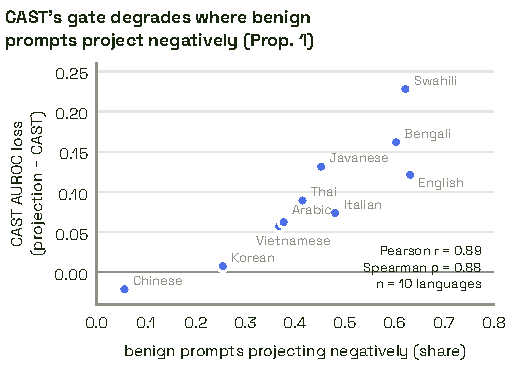
\includegraphics[width=0.62\linewidth]{figs/fig3_cast_sign.pdf}
\caption{Gate level, Tiny Aya Global: per-language AUROC loss when gating with CAST's cosine-tanh score instead of the projection (English-fit direction, layer \CondLayer, held-out activations), against the share of benign prompts with negative projection; $n=10$ languages, descriptive.}
\label{fig:castgate}
\end{figure}
\begin{figure}[!htbp]
\centering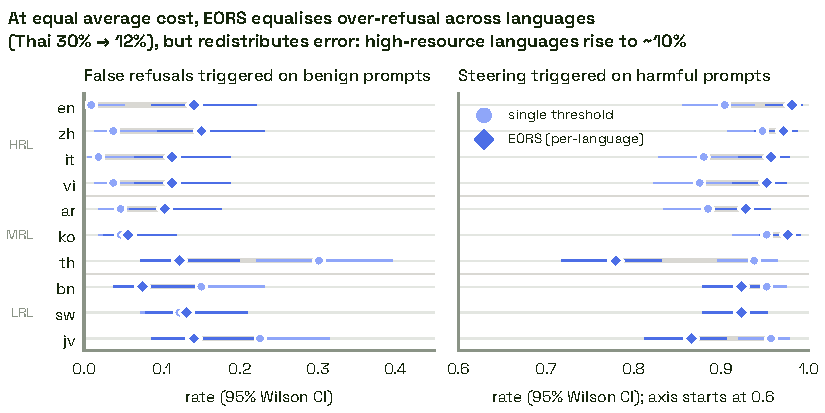
\includegraphics[width=\linewidth]{figs/fig2_gate_parity_eps0.1.pdf}
\caption{Gate-level parity on held-out activations (Tiny Aya Global, layer \CondLayer). At calibration-matched average cost, EORS ($\varepsilon=0.10$) reduces the worst-language false-fire rate from \MatchMaxFprSingle{} to \MatchMaxFprEors{} and raises high-resource languages to \MatchHrlFprEorsMin--\MatchHrlFprEorsMax{}; post hoc. Whiskers: 95\% Wilson intervals.}
\label{fig:gates}
\end{figure}
\begin{figure}[!htbp]
\centering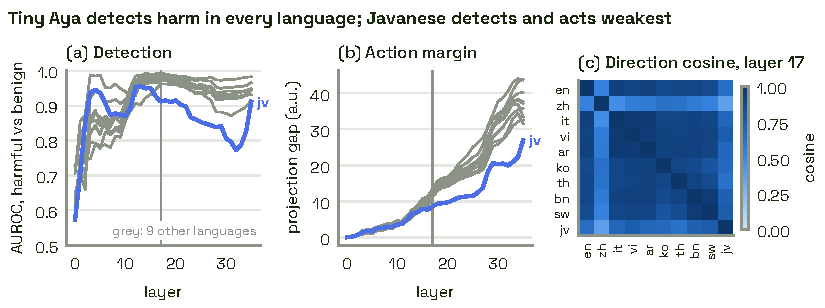
\includegraphics[width=\linewidth]{figs/fig1_detection_action.pdf}
\caption{Tiny Aya Global, held-out prompts: (a) AUROC of the pooled harm direction by layer (best layer \BestLayer: \AurocMinNonJv--\AurocMax{} in nine languages, Javanese \AurocJv); (b) projection gap; (c) cosine between language-specific refusal directions (mean \CosMean). Harm is represented in every language; the gate fires on \FailEors{} of the harmful prompts B0 answered harmfully.}
\label{fig:mech}
\end{figure}
\begin{figure}[!htbp]
\centering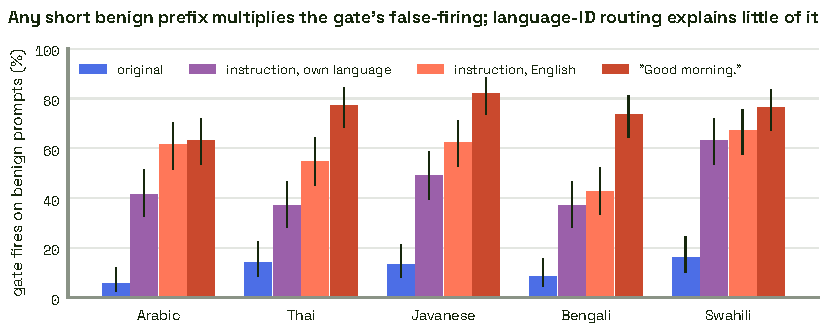
\includegraphics[width=\linewidth]{figs/figA_brittleness.pdf}
\caption{Gate-level false-firing of the EORS gate ($\varepsilon=0.10$, Tiny Aya Earth) on 106 benign test prompts per language, as is or with a benign prefix; 95\% Wilson intervals; constrained GlotLID picks the threshold on the modified prompt, as at inference. Post hoc.}
\label{fig:brittle}
\end{figure}

\begin{table}[!htbp]
\caption{Table~\ref{tab:arms} under the second judge, Gemini~3.5 Flash (broad rubric); unlabelled rows dropped.}
\label{tab:arms-gem}
\centering\resizebox{\linewidth}{!}{% AUTO-GENERATED by src/paper_numbers.py from runs/arms_report.json (gem)
\begin{tabular}{@{}llccc@{}}
\toprule
Arm & Gate / change & $\Delta$ mean SRR & $\Delta$ worst-language BRR & $\Delta$ mean HRR \\
\midrule
G-POOL & single pooled threshold & $+4.1$ {\scriptsize[$+2.7$, $+5.6$]} & $+30.2$ {\scriptsize[$+23.6$, $+40.6$]} & $+35.2$ {\scriptsize[$+30.8$, $+39.7$]} \\
G-EN & English vector, projection gate & $+4.1$ {\scriptsize[$+2.8$, $+5.6$]} & $+31.4$ {\scriptsize[$+24.4$, $+42.0$]} & $+37.1$ {\scriptsize[$+32.4$, $+41.9$]} \\
CAST-EN & English vector, CAST gate & $+3.9$ {\scriptsize[$+2.6$, $+5.5$]} & $+27.4$ {\scriptsize[$+19.8$, $+35.8$]} & $+35.2$ {\scriptsize[$+30.7$, $+39.9$]} \\
G-CAL & per-language max-F1 & $+4.1$ {\scriptsize[$+2.7$, $+5.6$]} & $+23.8$ {\scriptsize[$+17.9$, $+32.9$]} & $+35.0$ {\scriptsize[$+30.6$, $+39.5$]} \\
EORS $\varepsilon{=}.10$ & per-language conformal & $+4.0$ {\scriptsize[$+2.6$, $+5.5$]} & $+11.3$ {\scriptsize[$+6.6$, $+17.9$]} & $+33.0$ {\scriptsize[$+28.7$, $+37.4$]} \\
EORS $\varepsilon{=}.05$ & per-language conformal & $+3.5$ {\scriptsize[$+2.3$, $+4.9$]} & $+7.5$ {\scriptsize[$+2.8$, $+12.3$]} & $+26.6$ {\scriptsize[$+22.7$, $+30.8$]} \\
ReSta & weight arithmetic & $+0.8$ {\scriptsize[$-0.4$, $+2.0$]} & $+17.0$ {\scriptsize[$+9.4$, $+25.5$]} & $+7.5$ {\scriptsize[$+5.4$, $+9.7$]} \\
NEG & negative control & $-3.2$ {\scriptsize[$-4.6$, $-1.9$]} & $-1.9$ {\scriptsize[$-6.6$, $+4.7$]} & $-2.8$ {\scriptsize[$-4.8$, $-0.8$]} \\
\midrule
B1 (no preamble) & vs.\ B0, Tiny Aya Global & $-0.0$ {\scriptsize[$-0.8$, $+0.7$]} & $+3.8$ {\scriptsize[$-1.9$, $+9.4$]} & $+1.6$ {\scriptsize[$+0.4$, $+2.9$]} \\
\bottomrule
\end{tabular}
}
\end{table}

\section{Baseline and natural drift}
\label{app:drift}
Before any repair: the baseline outcomes of Tiny Aya Global by language (Figure~\ref{fig:baseline}), and the natural drift from Global to its regional sibling Earth, the model every repair arm starts from (Figure~\ref{fig:drift}).
\begin{figure}[!htbp]
\centering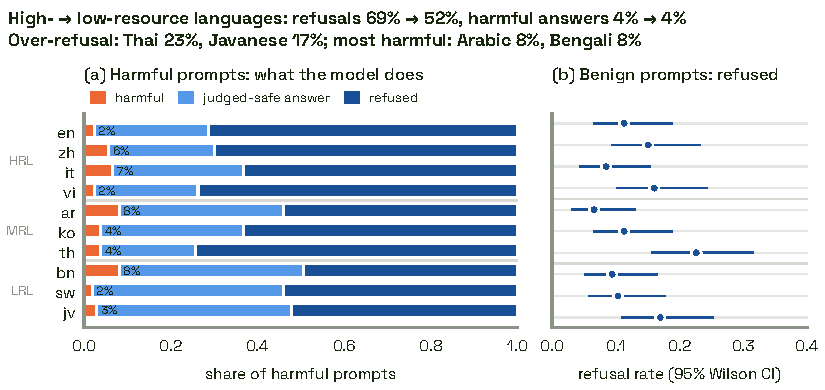
\includegraphics[width=\linewidth]{figs/fig4_baseline_outcomes_q3g4b.pdf}
\caption{Baseline B0 (Tiny Aya Global): outcomes on harmful prompts and refusal of benign prompts by language, Qwen3Guard-4B; refusal falls from high- to low-resource languages (\BZeroQRefHrl{} to \BZeroQRefLrl) while the harmful share is flat under this judge (\BZeroQHarmHrl{} in both tiers) and rises under Gemini (\BZeroGHarmHrl{} to \BZeroGHarmLrl).}
\label{fig:baseline}
\end{figure}
\begin{figure}[!htbp]
\centering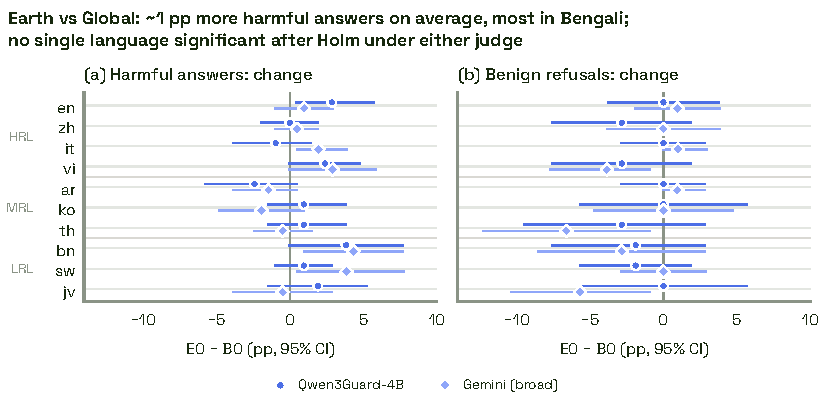
\includegraphics[width=\linewidth]{figs/fig5_drift_B0_E0.pdf}
\caption{Natural drift: Tiny Aya Earth minus Global, paired per-language differences with 95\% bootstrap intervals; circles Qwen3Guard-4B, diamonds Gemini. Exact McNemar tests, Holm-corrected; none significant.}
\label{fig:drift}
\end{figure}

\section{Circuit discovery: a negative result and tooling notes}
\label{app:circuits}
We attempted to localise refusal with CircuitKIT's node-level EAP-IG on en, sw and bn, holding to the faithfulness standard of~\citet{hanna2024faith}: circuit overlap is not evidence of shared mechanism; faithfulness is. The TransformerLens port passes CircuitKIT's parity gate (maximum next-token KL $\CkParityMaxKl$). Discovery needs \CkPeakMin--\CkPeakMax{}\,GiB of GPU memory at chat-template length, beyond a T4 or L4, and requires replacing TransformerLens's broadcast per-head output with an equivalent einsum. Harmful and benign prompts must be paired at equal token length, because CircuitKIT left-pads pairs and the safety preamble precedes the user turn.
With length-matched pairs, held-out patching faithfulness is at most \CkFaithTwentyMax{} with up to 20\% of the \CkNodes{} nodes, \CkFaithFortyMin--\CkFaithFortyMax{} at 40\%, \CkFaithSixtyMin--\CkFaithSixtyMax{} at 60\%, and \CkFaithFull{} with all nodes (a sanity check). Our pre-fixed criterion (faithfulness $\geq 0.5$ at $\leq 40\%$ of nodes) is not met, so we make no circuit claims: under this metric, refusal on these prompts is not carried by a sparse node-level circuit. SafeTune's circuit-to-layer adapter, given the top 20\% of nodes, selects nearly every layer, so circuit-guided layer choice was uninformative here.

\clearpage
\section*{NeurIPS Paper Checklist}



\begin{enumerate}

\item {\bf Claims}
    \item[] Question: Do the main claims made in the abstract and introduction accurately reflect the paper's contributions and scope?
    \item[] Answer: \answerYes{}
    \item[] Justification: The abstract and introduction state the three findings of \S\ref{sec:results} with their scope (one model family, translated benign prompts) and the trade-off the first one implies.
    \item[] Guidelines:
    \begin{itemize}
        \item The answer \answerNA{} means that the abstract and introduction do not include the claims made in the paper.
        \item The abstract and/or introduction should clearly state the claims made, including the contributions made in the paper and important assumptions and limitations. A \answerNo{} or \answerNA{} answer to this question will not be perceived well by the reviewers. 
        \item The claims made should match theoretical and experimental results, and reflect how much the results can be expected to generalize to other settings. 
        \item It is fine to include aspirational goals as motivation as long as it is clear that these goals are not attained by the paper. 
    \end{itemize}

\item {\bf Limitations}
    \item[] Question: Does the paper discuss the limitations of the work performed by the authors?
    \item[] Answer: \answerYes{}
    \item[] Justification: \S\ref{sec:limitations} lists the limitations, including one model family, judges not validated in the low-resource tier, a single pre-registered calibration split, and reused test prompts.
    \item[] Guidelines:
    \begin{itemize}
        \item The answer \answerNA{} means that the paper has no limitation while the answer \answerNo{} means that the paper has limitations, but those are not discussed in the paper. 
        \item The authors are encouraged to create a separate ``Limitations'' section in their paper.
        \item The paper should point out any strong assumptions and how robust the results are to violations of these assumptions (e.g., independence assumptions, noiseless settings, model well-specification, asymptotic approximations only holding locally). The authors should reflect on how these assumptions might be violated in practice and what the implications would be.
        \item The authors should reflect on the scope of the claims made, e.g., if the approach was only tested on a few datasets or with a few runs. In general, empirical results often depend on implicit assumptions, which should be articulated.
        \item The authors should reflect on the factors that influence the performance of the approach. For example, a facial recognition algorithm may perform poorly when image resolution is low or images are taken in low lighting. Or a speech-to-text system might not be used reliably to provide closed captions for online lectures because it fails to handle technical jargon.
        \item The authors should discuss the computational efficiency of the proposed algorithms and how they scale with dataset size.
        \item If applicable, the authors should discuss possible limitations of their approach to address problems of privacy and fairness.
        \item While the authors might fear that complete honesty about limitations might be used by reviewers as grounds for rejection, a worse outcome might be that reviewers discover limitations that aren't acknowledged in the paper. The authors should use their best judgment and recognize that individual actions in favor of transparency play an important role in developing norms that preserve the integrity of the community. Reviewers will be specifically instructed to not penalize honesty concerning limitations.
    \end{itemize}

\item {\bf Theory assumptions and proofs}
    \item[] Question: For each theoretical result, does the paper provide the full set of assumptions and a complete (and correct) proof?
    \item[] Answer: \answerYes{}
    \item[] Justification: Remark~\ref{prop:cast} states its linear-regime assumption, which \S\ref{sec:method} checks on the model's activations; Prop.~\ref{prop:eors} is the standard split-conformal result with its assumptions (independent score fit, exchangeability, correct language identification) stated and cited.
    \item[] Guidelines:
    \begin{itemize}
        \item The answer \answerNA{} means that the paper does not include theoretical results. 
        \item All the theorems, formulas, and proofs in the paper should be numbered and cross-referenced.
        \item All assumptions should be clearly stated or referenced in the statement of any theorems.
        \item The proofs can either appear in the main paper or the supplemental material, but if they appear in the supplemental material, the authors are encouraged to provide a short proof sketch to provide intuition. 
        \item Inversely, any informal proof provided in the core of the paper should be complemented by formal proofs provided in appendix or supplemental material.
        \item Theorems and Lemmas that the proof relies upon should be properly referenced. 
    \end{itemize}

    \item {\bf Experimental result reproducibility}
    \item[] Question: Does the paper fully disclose all the information needed to reproduce the main experimental results of the paper to the extent that it affects the main claims and/or conclusions of the paper (regardless of whether the code and data are provided or not)?
    \item[] Answer: \answerYes{}
    \item[] Justification: \S\ref{sec:setting}--\ref{sec:method} and Appendix~\ref{app:prereg} give data construction, model versions, arm fitting, seeds, decoding and the analysis plan; every number in the paper is generated by script from released result files.
    \item[] Guidelines:
    \begin{itemize}
        \item The answer \answerNA{} means that the paper does not include experiments.
        \item If the paper includes experiments, a \answerNo{} answer to this question will not be perceived well by the reviewers: Making the paper reproducible is important, regardless of whether the code and data are provided or not.
        \item If the contribution is a dataset and\slash or model, the authors should describe the steps taken to make their results reproducible or verifiable. 
        \item Depending on the contribution, reproducibility can be accomplished in various ways. For example, if the contribution is a novel architecture, describing the architecture fully might suffice, or if the contribution is a specific model and empirical evaluation, it may be necessary to either make it possible for others to replicate the model with the same dataset, or provide access to the model. In general. releasing code and data is often one good way to accomplish this, but reproducibility can also be provided via detailed instructions for how to replicate the results, access to a hosted model (e.g., in the case of a large language model), releasing of a model checkpoint, or other means that are appropriate to the research performed.
        \item While NeurIPS does not require releasing code, the conference does require all submissions to provide some reasonable avenue for reproducibility, which may depend on the nature of the contribution. For example
        \begin{enumerate}
            \item If the contribution is primarily a new algorithm, the paper should make it clear how to reproduce that algorithm.
            \item If the contribution is primarily a new model architecture, the paper should describe the architecture clearly and fully.
            \item If the contribution is a new model (e.g., a large language model), then there should either be a way to access this model for reproducing the results or a way to reproduce the model (e.g., with an open-source dataset or instructions for how to construct the dataset).
            \item We recognize that reproducibility may be tricky in some cases, in which case authors are welcome to describe the particular way they provide for reproducibility. In the case of closed-source models, it may be that access to the model is limited in some way (e.g., to registered users), but it should be possible for other researchers to have some path to reproducing or verifying the results.
        \end{enumerate}
    \end{itemize}


\item {\bf Open access to data and code}
    \item[] Question: Does the paper provide open access to the data and code, with sufficient instructions to faithfully reproduce the main experimental results, as described in supplemental material?
    \item[] Answer: \answerYes{}
    \item[] Justification: Code (Apache-2.0), prompts, judge labels and aggregates will be released openly with the paper; model responses and steering artifacts, which are dual-use, will be released under gated access with documented terms.
    \item[] Guidelines:
    \begin{itemize}
        \item The answer \answerNA{} means that paper does not include experiments requiring code.
        \item Please see the NeurIPS code and data submission guidelines (\url{https://neurips.cc/public/guides/CodeSubmissionPolicy}) for more details.
        \item While we encourage the release of code and data, we understand that this might not be possible, so \answerNo{} is an acceptable answer. Papers cannot be rejected simply for not including code, unless this is central to the contribution (e.g., for a new open-source benchmark).
        \item The instructions should contain the exact command and environment needed to run to reproduce the results. See the NeurIPS code and data submission guidelines (\url{https://neurips.cc/public/guides/CodeSubmissionPolicy}) for more details.
        \item The authors should provide instructions on data access and preparation, including how to access the raw data, preprocessed data, intermediate data, and generated data, etc.
        \item The authors should provide scripts to reproduce all experimental results for the new proposed method and baselines. If only a subset of experiments are reproducible, they should state which ones are omitted from the script and why.
        \item At submission time, to preserve anonymity, the authors should release anonymized versions (if applicable).
        \item Providing as much information as possible in supplemental material (appended to the paper) is recommended, but including URLs to data and code is permitted.
    \end{itemize}


\item {\bf Experimental setting/details}
    \item[] Question: Does the paper specify all the training and test details (e.g., data splits, hyperparameters, how they were chosen, type of optimizer) necessary to understand the results?
    \item[] Answer: \answerYes{}
    \item[] Justification: \S\ref{sec:setting}--\ref{sec:method} specify the splits (calibration/test by prompt id; fit/conformal fold by seeded permutation), thresholds, steering strength rule, layers and judges.
    \item[] Guidelines:
    \begin{itemize}
        \item The answer \answerNA{} means that the paper does not include experiments.
        \item The experimental setting should be presented in the core of the paper to a level of detail that is necessary to appreciate the results and make sense of them.
        \item The full details can be provided either with the code, in appendix, or as supplemental material.
    \end{itemize}

\item {\bf Experiment statistical significance}
    \item[] Question: Does the paper report error bars suitably and correctly defined or other appropriate information about the statistical significance of the experiments?
    \item[] Answer: \answerYes{}
    \item[] Justification: All comparisons report 95\% paired bootstrap intervals over prompt ids (the sampling unit), exact McNemar tests with Holm correction per language, Holm correction across budgets for the co-primary estimands, and Wilson intervals for rates (\S\ref{sec:setting}).
    \item[] Guidelines:
    \begin{itemize}
        \item The answer \answerNA{} means that the paper does not include experiments.
        \item The authors should answer \answerYes{} if the results are accompanied by error bars, confidence intervals, or statistical significance tests, at least for the experiments that support the main claims of the paper.
        \item The factors of variability that the error bars are capturing should be clearly stated (for example, train/test split, initialization, random drawing of some parameter, or overall run with given experimental conditions).
        \item The method for calculating the error bars should be explained (closed form formula, call to a library function, bootstrap, etc.)
        \item The assumptions made should be given (e.g., Normally distributed errors).
        \item It should be clear whether the error bar is the standard deviation or the standard error of the mean.
        \item It is OK to report 1-sigma error bars, but one should state it. The authors should preferably report a 2-sigma error bar than state that they have a 96\% CI, if the hypothesis of Normality of errors is not verified.
        \item For asymmetric distributions, the authors should be careful not to show in tables or figures symmetric error bars that would yield results that are out of range (e.g., negative error rates).
        \item If error bars are reported in tables or plots, the authors should explain in the text how they were calculated and reference the corresponding figures or tables in the text.
    \end{itemize}

\item {\bf Experiments compute resources}
    \item[] Question: For each experiment, does the paper provide sufficient information on the computer resources (type of compute workers, memory, time of execution) needed to reproduce the experiments?
    \item[] Answer: \answerYes{}
    \item[] Justification: \S\ref{sec:setting} reports A100 time per arm for generation and scoring; activations and analyses ran on an Apple M1 Pro laptop.
    \item[] Guidelines:
    \begin{itemize}
        \item The answer \answerNA{} means that the paper does not include experiments.
        \item The paper should indicate the type of compute workers CPU or GPU, internal cluster, or cloud provider, including relevant memory and storage.
        \item The paper should provide the amount of compute required for each of the individual experimental runs as well as estimate the total compute. 
        \item The paper should disclose whether the full research project required more compute than the experiments reported in the paper (e.g., preliminary or failed experiments that didn't make it into the paper). 
    \end{itemize}
    
\item {\bf Code of ethics}
    \item[] Question: Does the research conducted in the paper conform, in every respect, with the NeurIPS Code of Ethics \url{https://neurips.cc/public/EthicsGuidelines}?
    \item[] Answer: \answerYes{}
    \item[] Justification: The work uses public benchmarks, releases no new attack content, gates dual-use artifacts, and follows the NeurIPS Code of Ethics.
    \item[] Guidelines:
    \begin{itemize}
        \item The answer \answerNA{} means that the authors have not reviewed the NeurIPS Code of Ethics.
        \item If the authors answer \answerNo, they should explain the special circumstances that require a deviation from the Code of Ethics.
        \item The authors should make sure to preserve anonymity (e.g., if there is a special consideration due to laws or regulations in their jurisdiction).
    \end{itemize}


\item {\bf Broader impacts}
    \item[] Question: Does the paper discuss both potential positive societal impacts and negative societal impacts of the work performed?
    \item[] Answer: \answerYes{}
    \item[] Justification: The Broader impact section discusses benefits for speakers of low-resource languages and the misuse risk of steering artifacts and the brittleness result.
    \item[] Guidelines:
    \begin{itemize}
        \item The answer \answerNA{} means that there is no societal impact of the work performed.
        \item If the authors answer \answerNA{} or \answerNo, they should explain why their work has no societal impact or why the paper does not address societal impact.
        \item Examples of negative societal impacts include potential malicious or unintended uses (e.g., disinformation, generating fake profiles, surveillance), fairness considerations (e.g., deployment of technologies that could make decisions that unfairly impact specific groups), privacy considerations, and security considerations.
        \item The conference expects that many papers will be foundational research and not tied to particular applications, let alone deployments. However, if there is a direct path to any negative applications, the authors should point it out. For example, it is legitimate to point out that an improvement in the quality of generative models could be used to generate Deepfakes for disinformation. On the other hand, it is not needed to point out that a generic algorithm for optimizing neural networks could enable people to train models that generate Deepfakes faster.
        \item The authors should consider possible harms that could arise when the technology is being used as intended and functioning correctly, harms that could arise when the technology is being used as intended but gives incorrect results, and harms following from (intentional or unintentional) misuse of the technology.
        \item If there are negative societal impacts, the authors could also discuss possible mitigation strategies (e.g., gated release of models, providing defenses in addition to attacks, mechanisms for monitoring misuse, mechanisms to monitor how a system learns from feedback over time, improving the efficiency and accessibility of ML).
    \end{itemize}
    
\item {\bf Safeguards}
    \item[] Question: Does the paper describe safeguards that have been put in place for responsible release of data or models that have a high risk for misuse (e.g., pre-trained language models, image generators, or scraped datasets)?
    \item[] Answer: \answerYes{}
    \item[] Justification: Model responses (some harmful) and steering vectors, which can be inverted to remove refusal, will be released only through gated repositories with a research-use agreement and a content warning.
    \item[] Guidelines:
    \begin{itemize}
        \item The answer \answerNA{} means that the paper poses no such risks.
        \item Released models that have a high risk for misuse or dual-use should be released with necessary safeguards to allow for controlled use of the model, for example by requiring that users adhere to usage guidelines or restrictions to access the model or implementing safety filters. 
        \item Datasets that have been scraped from the Internet could pose safety risks. The authors should describe how they avoided releasing unsafe images.
        \item We recognize that providing effective safeguards is challenging, and many papers do not require this, but we encourage authors to take this into account and make a best faith effort.
    \end{itemize}

\item {\bf Licenses for existing assets}
    \item[] Question: Are the creators or original owners of assets (e.g., code, data, models), used in the paper, properly credited and are the license and terms of use explicitly mentioned and properly respected?
    \item[] Answer: \answerYes{}
    \item[] Justification: \S\ref{sec:setting} names each source and its licence (MultiJail MIT; XSTest and PolyGuardPrompts CC-BY-4.0; Aya red-teaming Apache-2.0; Tiny Aya and NLLB CC-BY-NC-4.0) and cites the creators.
    \item[] Guidelines:
    \begin{itemize}
        \item The answer \answerNA{} means that the paper does not use existing assets.
        \item The authors should cite the original paper that produced the code package or dataset.
        \item The authors should state which version of the asset is used and, if possible, include a URL.
        \item The name of the license (e.g., CC-BY 4.0) should be included for each asset.
        \item For scraped data from a particular source (e.g., website), the copyright and terms of service of that source should be provided.
        \item If assets are released, the license, copyright information, and terms of use in the package should be provided. For popular datasets, \url{paperswithcode.com/datasets} has curated licenses for some datasets. Their licensing guide can help determine the license of a dataset.
        \item For existing datasets that are re-packaged, both the original license and the license of the derived asset (if it has changed) should be provided.
        \item If this information is not available online, the authors are encouraged to reach out to the asset's creators.
    \end{itemize}

\item {\bf New assets}
    \item[] Question: Are new assets introduced in the paper well documented and is the documentation provided alongside the assets?
    \item[] Answer: \answerYes{}
    \item[] Justification: The dataset and artifacts to be released carry datasheet-style cards (composition, collection, translation quality checks, intended and out-of-scope uses, licences, limitations).
    \item[] Guidelines:
    \begin{itemize}
        \item The answer \answerNA{} means that the paper does not release new assets.
        \item Researchers should communicate the details of the dataset\slash code\slash model as part of their submissions via structured templates. This includes details about training, license, limitations, etc. 
        \item The paper should discuss whether and how consent was obtained from people whose asset is used.
        \item At submission time, remember to anonymize your assets (if applicable). You can either create an anonymized URL or include an anonymized zip file.
    \end{itemize}

\item {\bf Crowdsourcing and research with human subjects}
    \item[] Question: For crowdsourcing experiments and research with human subjects, does the paper include the full text of instructions given to participants and screenshots, if applicable, as well as details about compensation (if any)? 
    \item[] Answer: \answerNA{}
    \item[] Justification: No new human-subject data were collected; judge validation uses the existing human labels of PolyGuardPrompts.
    \item[] Guidelines:
    \begin{itemize}
        \item The answer \answerNA{} means that the paper does not involve crowdsourcing nor research with human subjects.
        \item Including this information in the supplemental material is fine, but if the main contribution of the paper involves human subjects, then as much detail as possible should be included in the main paper. 
        \item According to the NeurIPS Code of Ethics, workers involved in data collection, curation, or other labor should be paid at least the minimum wage in the country of the data collector. 
    \end{itemize}

\item {\bf Institutional review board (IRB) approvals or equivalent for research with human subjects}
    \item[] Question: Does the paper describe potential risks incurred by study participants, whether such risks were disclosed to the subjects, and whether Institutional Review Board (IRB) approvals (or an equivalent approval/review based on the requirements of your country or institution) were obtained?
    \item[] Answer: \answerNA{}
    \item[] Justification: No research with human subjects was conducted.
    \item[] Guidelines:
    \begin{itemize}
        \item The answer \answerNA{} means that the paper does not involve crowdsourcing nor research with human subjects.
        \item Depending on the country in which research is conducted, IRB approval (or equivalent) may be required for any human subjects research. If you obtained IRB approval, you should clearly state this in the paper. 
        \item We recognize that the procedures for this may vary significantly between institutions and locations, and we expect authors to adhere to the NeurIPS Code of Ethics and the guidelines for their institution. 
        \item For initial submissions, do not include any information that would break anonymity (if applicable), such as the institution conducting the review.
    \end{itemize}

\item {\bf Declaration of LLM usage}
    \item[] Question: Does the paper describe the usage of LLMs if it is an important, original, or non-standard component of the core methods in this research? Note that if the LLM is used only for writing, editing, or formatting purposes and does \emph{not} impact the core methodology, scientific rigor, or originality of the research, declaration is not required.
    %this research? 
    \item[] Answer: \answerYes{}
    \item[] Justification: LLMs are part of the method (Qwen3Guard and Gemini as judges, validated against human labels in \S\ref{sec:measure}), and implementation and drafting were a collaboration between the author and an AI agent, as the AI use disclosure describes.
    \item[] Guidelines:
    \begin{itemize}
        \item The answer \answerNA{} means that the core method development in this research does not involve LLMs as any important, original, or non-standard components.
        \item Please refer to our LLM policy in the NeurIPS handbook for what should or should not be described.
    \end{itemize}

\end{enumerate}
\end{document}
